%\documentclass[12pt,serif]{beamer}
%\documentclass[tikz,12pt,svgnames]{beamer}

%For printing
%\documentclass[table,handout,tikz,12pt,svgnames]{beamer}
%With animations
\documentclass[table,tikz,12pt,svgnames]{beamer}

\usepackage{CM-preamble}
\usepackage{gitdags}
\usepackage{subcaption}

\definecolor{darkgreen}{rgb}{0,0.6,0}
\definecolor{red}{rgb}{1,0,0}
\definecolor{green}{rgb}{0,1,0}
\definecolor{blue}{rgb}{0,0,1}
\definecolor{cyan}{rgb}{0.4,1,1}
\definecolor{orange}{rgb}{1,0.7,0}
\definecolor{dkgreen}{rgb}{0,0.6,0}
\definecolor{gray}{rgb}{0.5,0.5,0.5}
\definecolor{purple}{rgb}{0.58,0,0.82}
\definecolor{mintedbackground}{rgb}{0.95,0.95,0.95}
 
\title{\LARGE Gestion de versions}
\subtitle{avec \texttt{git}}
\date{}

%README TODO STUFF

\begin{document}

\begin{frame}
	\titlepage
\end{frame}

\begin{frame}
	\frametitle{Moi... \textit{\small (et ma décharge de responsabilité)}}
	\begin{itemize}
		\item Je suis étranger (hors UE)…
		\item J'ai un accent…
		\item Je me {\color{blue} trompe beaucoup} en français
		\begin{itemize}
			\item et en info, et en math, et \ldots
			\item n'hésitez pas à me corriger ou à me demander de répéter
		\end{itemize}
		\item Je commence à enseigner
		\begin{itemize}
			\item ce cours est tout nouveau
			\item j'accepte des critiques (constructives mais pas que)\\
			et surtout des recommandations
			\item n'hésitez pas à poser des questions
		\end{itemize}
		\item Je ne suis pas un expert
	\end{itemize}
\end{frame}


\begin{frame}
	\frametitle{Comment gérez-vous vos fichiers ?}
	\vspace{-1em}
	\begin{block}{}<1->
	\begin{itemize}
		\item Garder l'historique
		\item Partager
	\end{itemize}
	\end{block}
	\vspace{-2em}
	\begin{block}{}<2->
    \begin{adjustwidth}{-0.5cm}{-0.5cm}{}
		\begin{center}	
		{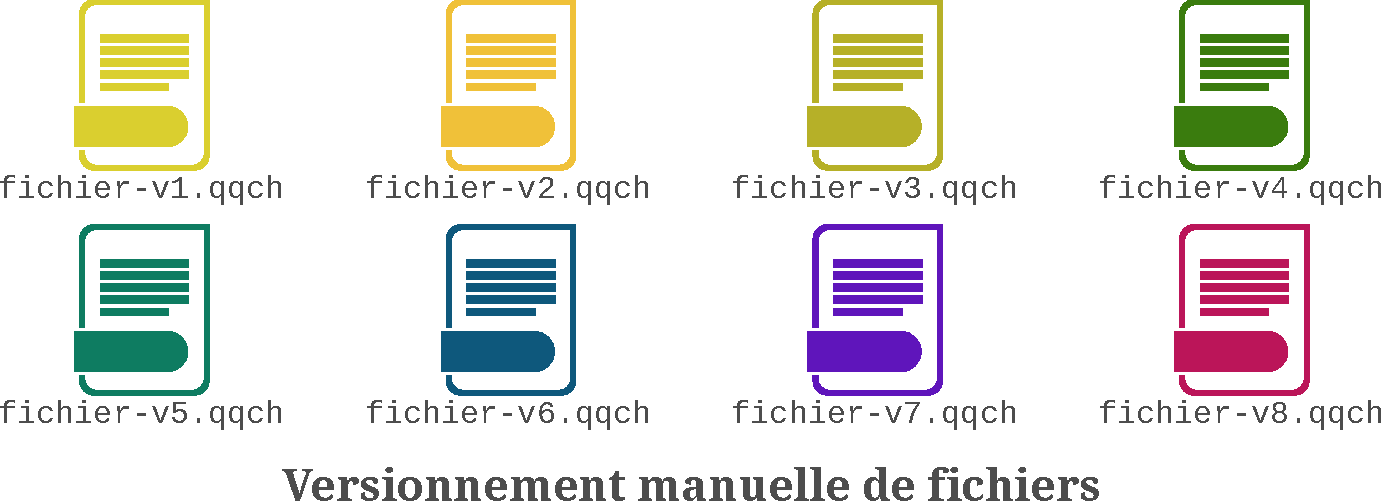
\includegraphics[scale=0.5]{images/file_versions.pdf}}
		\end{center}
	\end{adjustwidth}
	\end{block}
\end{frame}



\begin{frame}
	\frametitle{Comment collaborer sur un fichier ? }
	\vspace{-1em}
	\begin{block}{}
    \begin{adjustwidth}{-0.5cm}{-0.5cm}{}
		\begin{center}
		{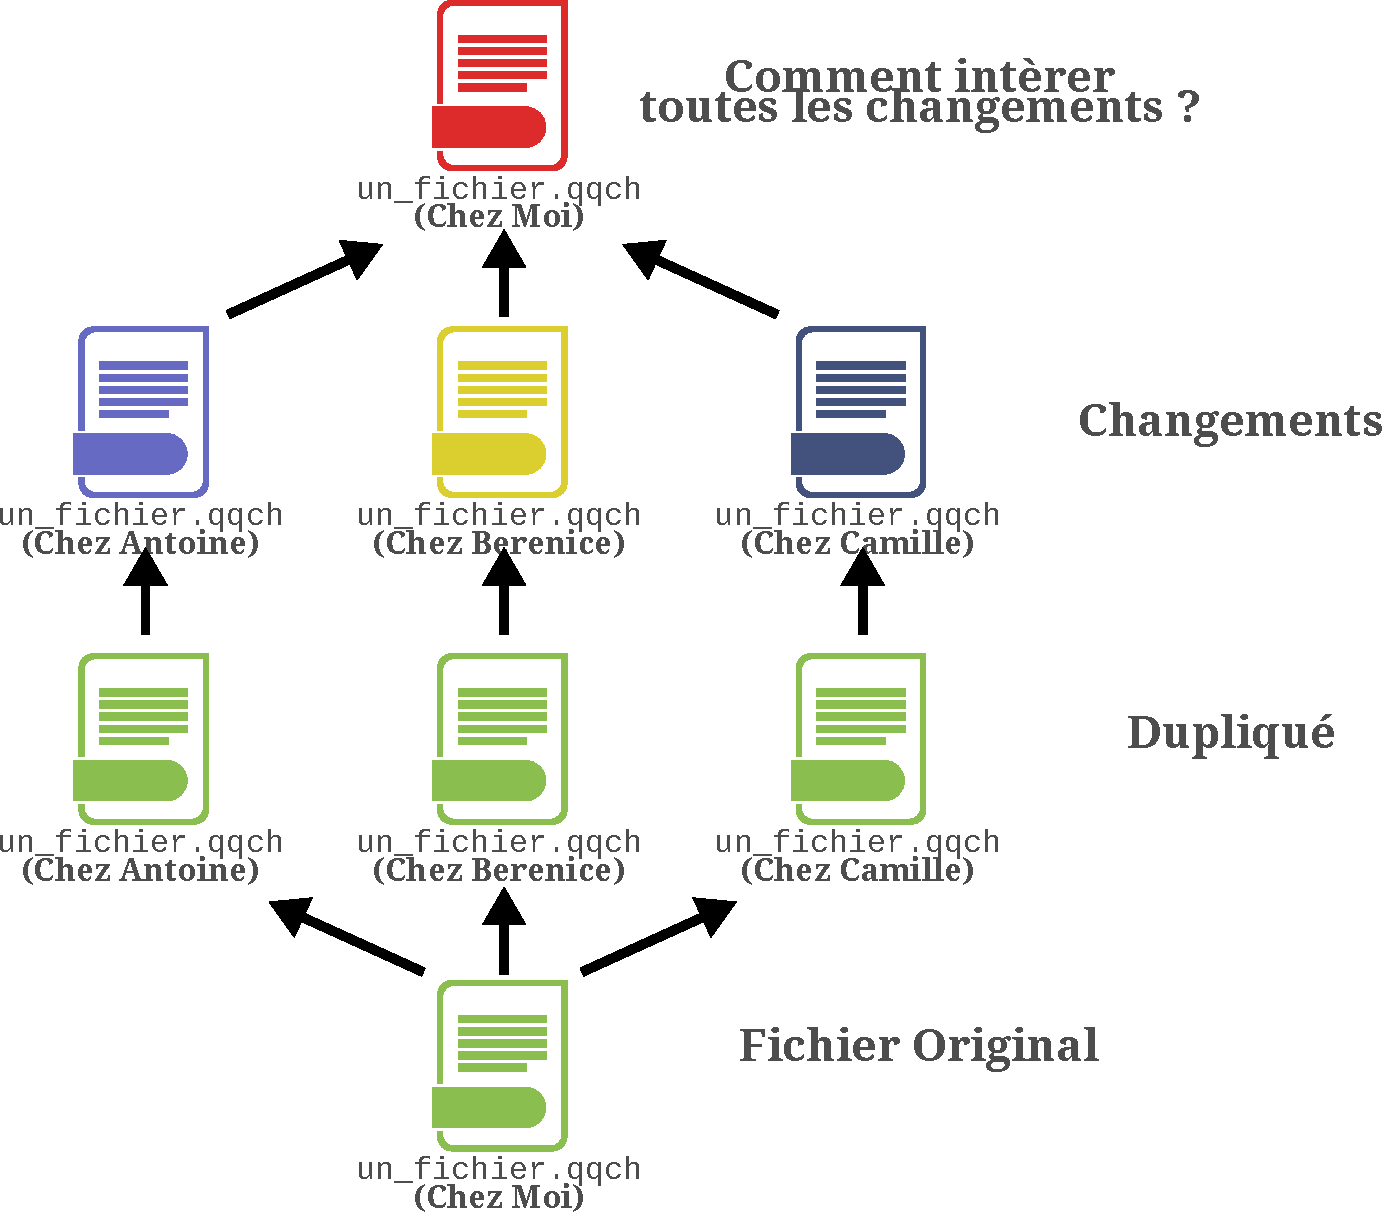
\includegraphics[scale=0.38]{images/file_share.pdf}}
		\end{center}
	\end{adjustwidth}
	\end{block}
\end{frame}


\begin{frame}
	\frametitle{Comment collaborer sur plusieurs fichiers ? }
%	\vspace{-4em}
	\begin{block}{}
    \begin{adjustwidth}{-0.5cm}{-0.5cm}{}
		\begin{center}
		{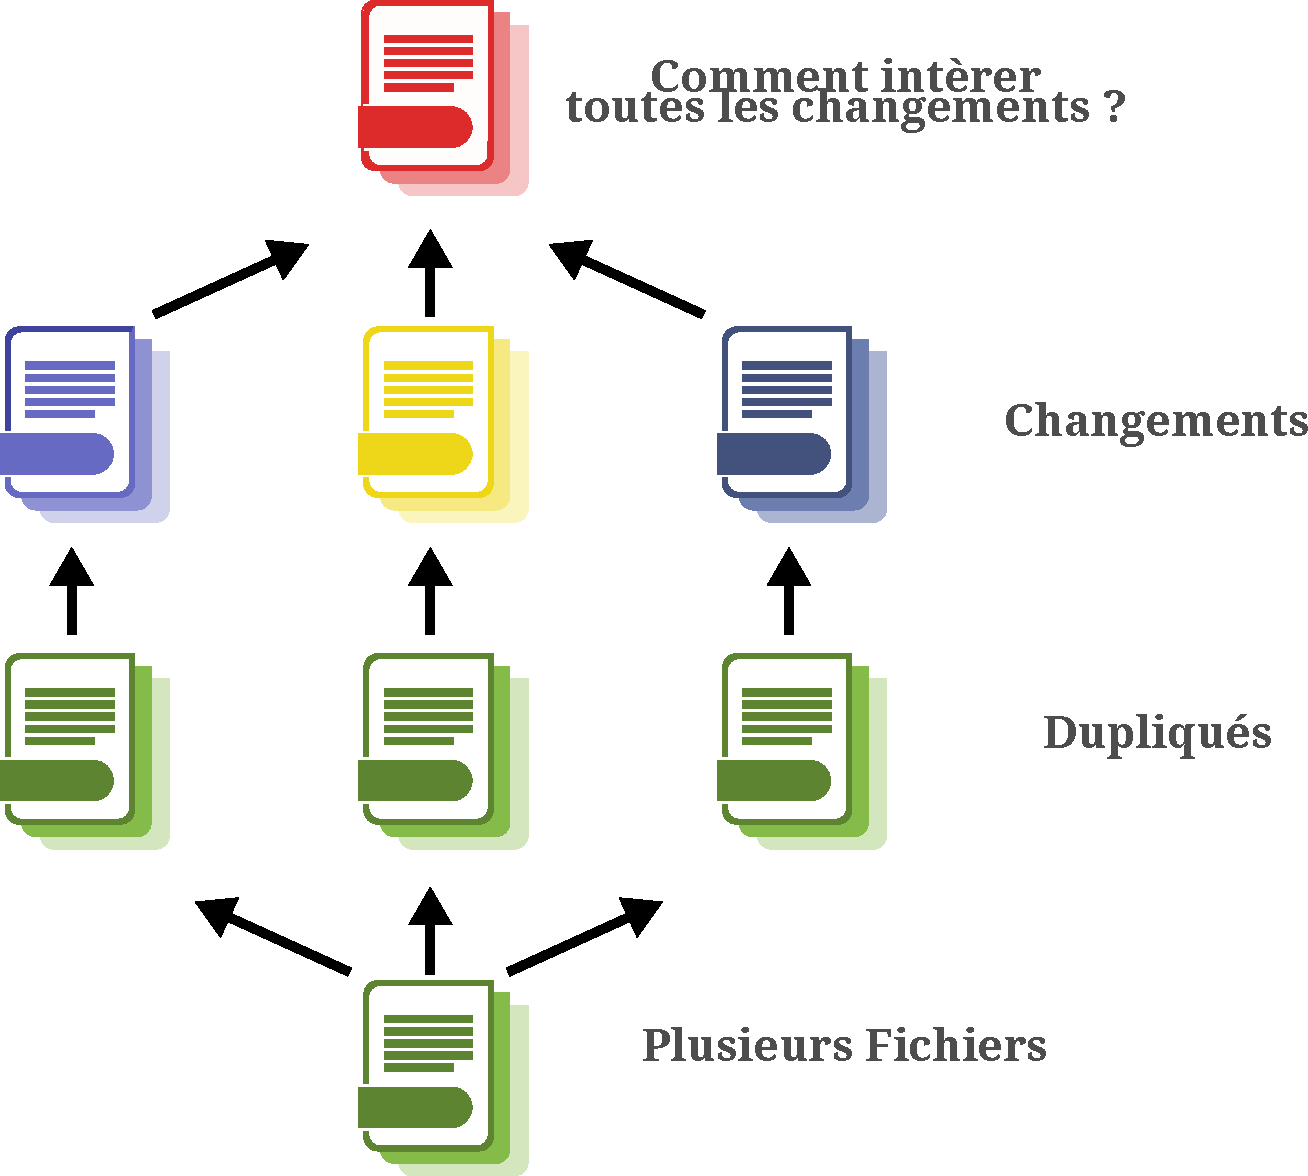
\includegraphics[scale=0.38]{images/file_share_many.pdf}}
		\end{center}
	\end{adjustwidth}
	\end{block}
\end{frame}


\begin{frame}
	\frametitle{D'autres solutions ? }
	\vspace{-4em}
	\begin{block}{}
    \begin{adjustwidth}{-0.5cm}{-0.5cm}{}
		\begin{center}
		{
\includegraphics[scale=0.43]{images/services.pdf}}
		\end{center}
	\end{adjustwidth}
	\end{block}
\end{frame}



\begin{frame}
	\frametitle{Gestion de versions}
		\begin{block}{}
%			\begin{itemize}
%				\item
				La \textbf{gestion de versions} (en anglais \textit{version control} ou \textit{revision control}) consiste à maintenir l'ensemble des versions d'un ou plusieurs fichiers (généralement en texte).
				Essentiellement utilisée dans le domaine de la création de logiciels, elle concerne surtout \textbf{la gestion des codes source}.
%			\end{itemize}
		\end{block}
		\begin{block}{}
		\small \url{https://fr.wikipedia.org/wiki/Gestion\_de\_versions}
		\end{block}
\end{frame}


\begin{frame}
	\frametitle{Gestion de versions}
	\vspace{-2em}
	\begin{block}{}
    \begin{adjustwidth}{-5.5cm}{-0.5cm}{}
		\begin{center}
		{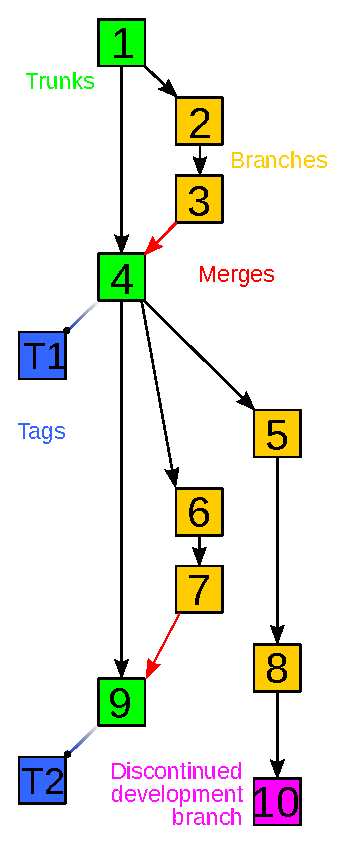
\includegraphics[scale=0.58]{images/gestion_versions.pdf}}
		\end{center}
	\end{adjustwidth}
	\vspace{-4em}
    \begin{adjustwidth}{5.0cm}{-1.5cm}{}
	\tiny Par Revision\_controlled\_project\_visualization.svg: *Subversion\_project\_visualization.svg: Traced by User:Stannered, original by en:User:Sami Keroladerivative work: Moxfyre (talk)derivative work: Echion2 (talk) — Revision\_controlled\_project\_visualization.svg, CC BY-SA 3.0, \url{https://commons.wikimedia.org/w/index.php?curid=9562807}
	\end{adjustwidth}
	\end{block}
\end{frame}

\begin{frame}
	\frametitle{Avantages de la gestion de versions}
	\begin{block}{}
    \begin{adjustwidth}{-0.3cm}{-1.4cm}{}
		\begin{itemize}
			\item Sauvegarde / Restauration
			\item Synchronisation du travail (partage, collaboration)
			\item Suivi de changements (très détaillé)
			\item Suivi de responsabilités / propriétaires / coupables
			\item \textit{Sandboxing} (espace confiné, environnement de test, isolation)
			\item \textit{Branching and merging}
			\item Passage à l'échelle (10, 100, 1.000, 10.000 développeurs)
		\end{itemize}
	\end{adjustwidth}
	\end{block}
\end{frame}

\begin{frame}
	\frametitle{Que mettre dans un Logiciel de Gestion de Versions ?}
	\vspace{-2em}
	\begin{block}{}%À mettre
    \begin{adjustwidth}{-0.5cm}{}
		\begin{itemize}
			\item Tous les sources du projet
			\begin{itemize}
				\item code source (\texttt{.c .cpp .java .py} \dots)
				\item scripts de build (\texttt{Makefile pom.xml} \ldots)
				\item Documentation (\texttt{.txt .tex Readme} \ldots)
				\item Ressources (images \ldots)
				\item Scripts divers (déploiement, \texttt{.sql, .sh} \ldots)
			\end{itemize}
		\end{itemize}
	\end{adjustwidth}	
	\end{block}
	\begin{block}{\color{red} À NE PAS mettre}<2->
    \begin{adjustwidth}{-0.5cm}{}
	\begin{itemize}
		\item Les fichiers générés
		\begin{itemize}
			\item Résultat de compilation (\texttt{.class .o .exe .jar} \ldots)
			\item Autres fichiers générés (\texttt{.ps .dvi .pdf javadoc} \ldots)
		\end{itemize}
	\end{itemize}
	\end{adjustwidth}
	\end{block}
\end{frame}

\begin{frame}
\frametitle{Why the \texttt{git} ?}
\begin{block}{C'est \textit{Ze Standard}}
	%    \begin{adjustwidth}{-0.9cm}{}
	\begin{itemize}
		\item \textit{git - the stupid content tracker}
		\item Outil professionnel
		\item Rapide, multi-plateforme, flexible
	\end{itemize}
%	\end{adjustwidth}
\end{block}
\begin{block}{\textit{To Share or Not to Share}}
	\begin{itemize}
		\item Enrichissez vos CV
		\begin{itemize}
			\item \url{https://github.com/}
		\end{itemize}
		\item Choisir sa licence
		\begin{itemize}
			\item Code --- GPL, Apache, BSD, MIT, Propriétaire \url{https://choosealicense.com/}
			\item Documents/Rapports --- Creative commons \url{https://creativecommons.org/}
		\end{itemize}
	\end{itemize}
\end{block}
\end{frame}

\begin{frame}
\frametitle{Concepts et commandes \texttt{git}}
\begin{adjustwidth}{-0.75cm}{0cm}{}
\vspace{-1em}
	\begin{center}
		\only<1>{{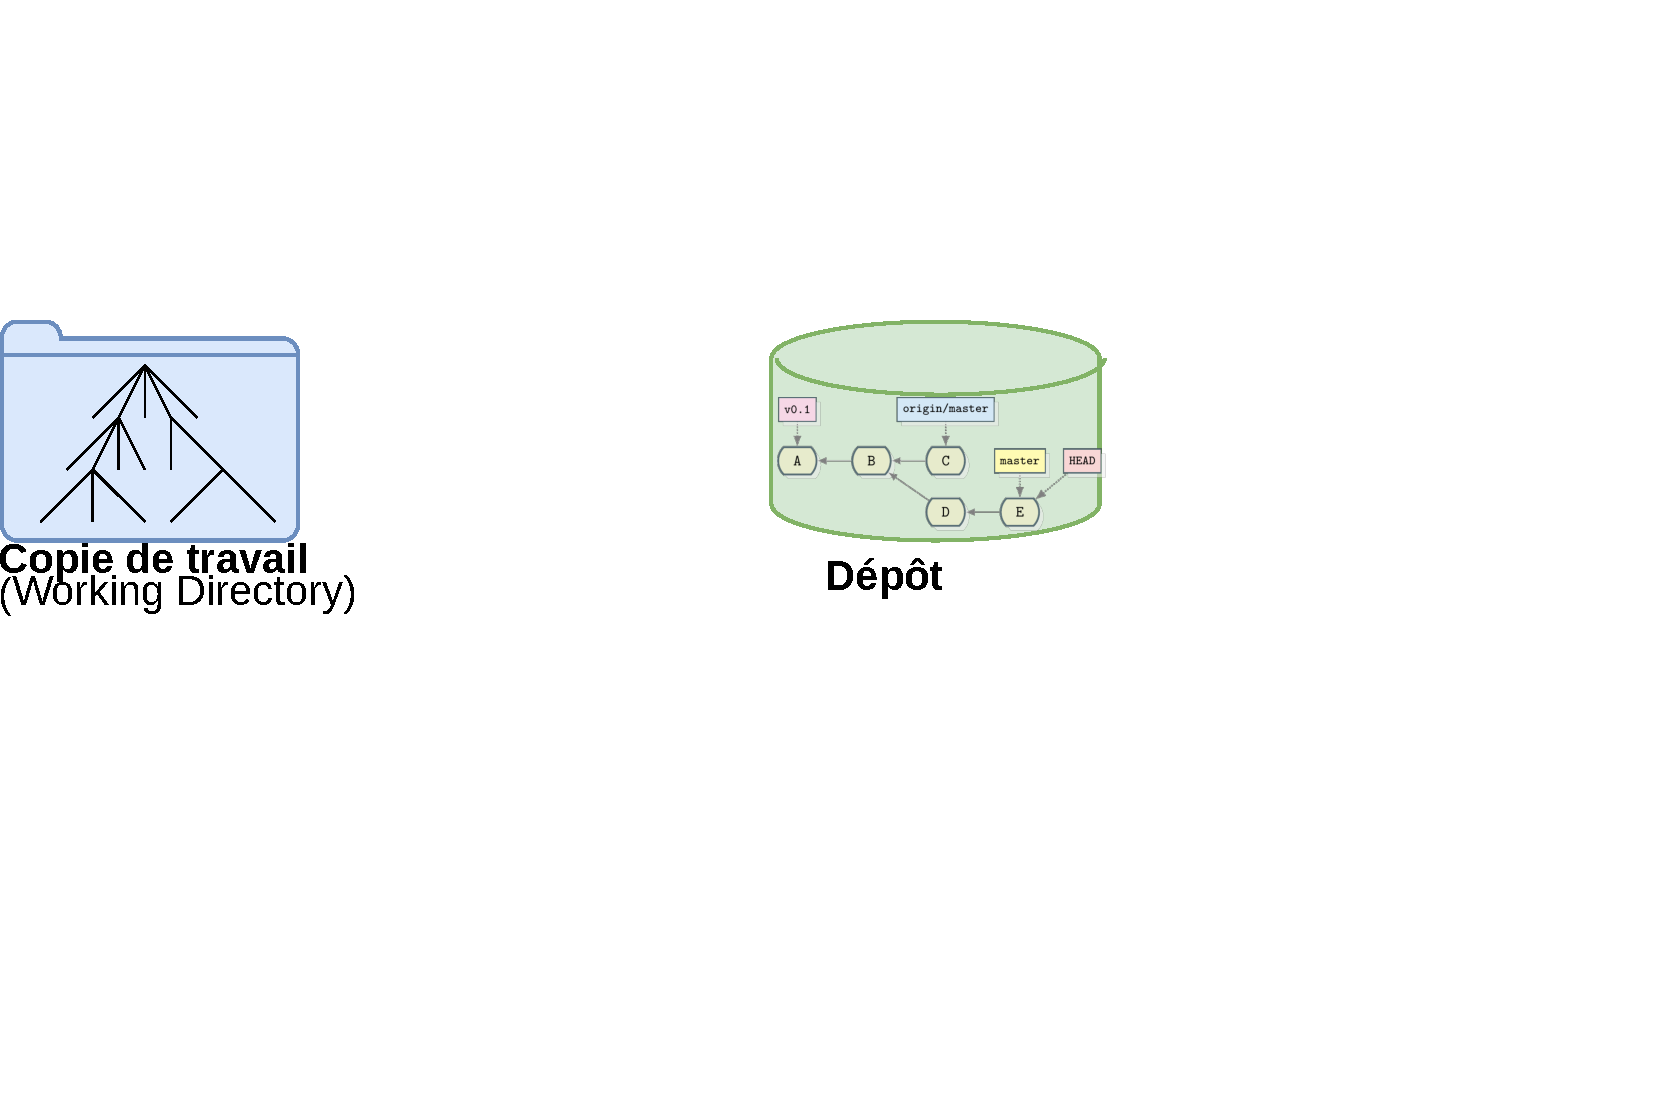
\includegraphics[scale=0.44]{images/workflow1.pdf}}}
		\only<2>{{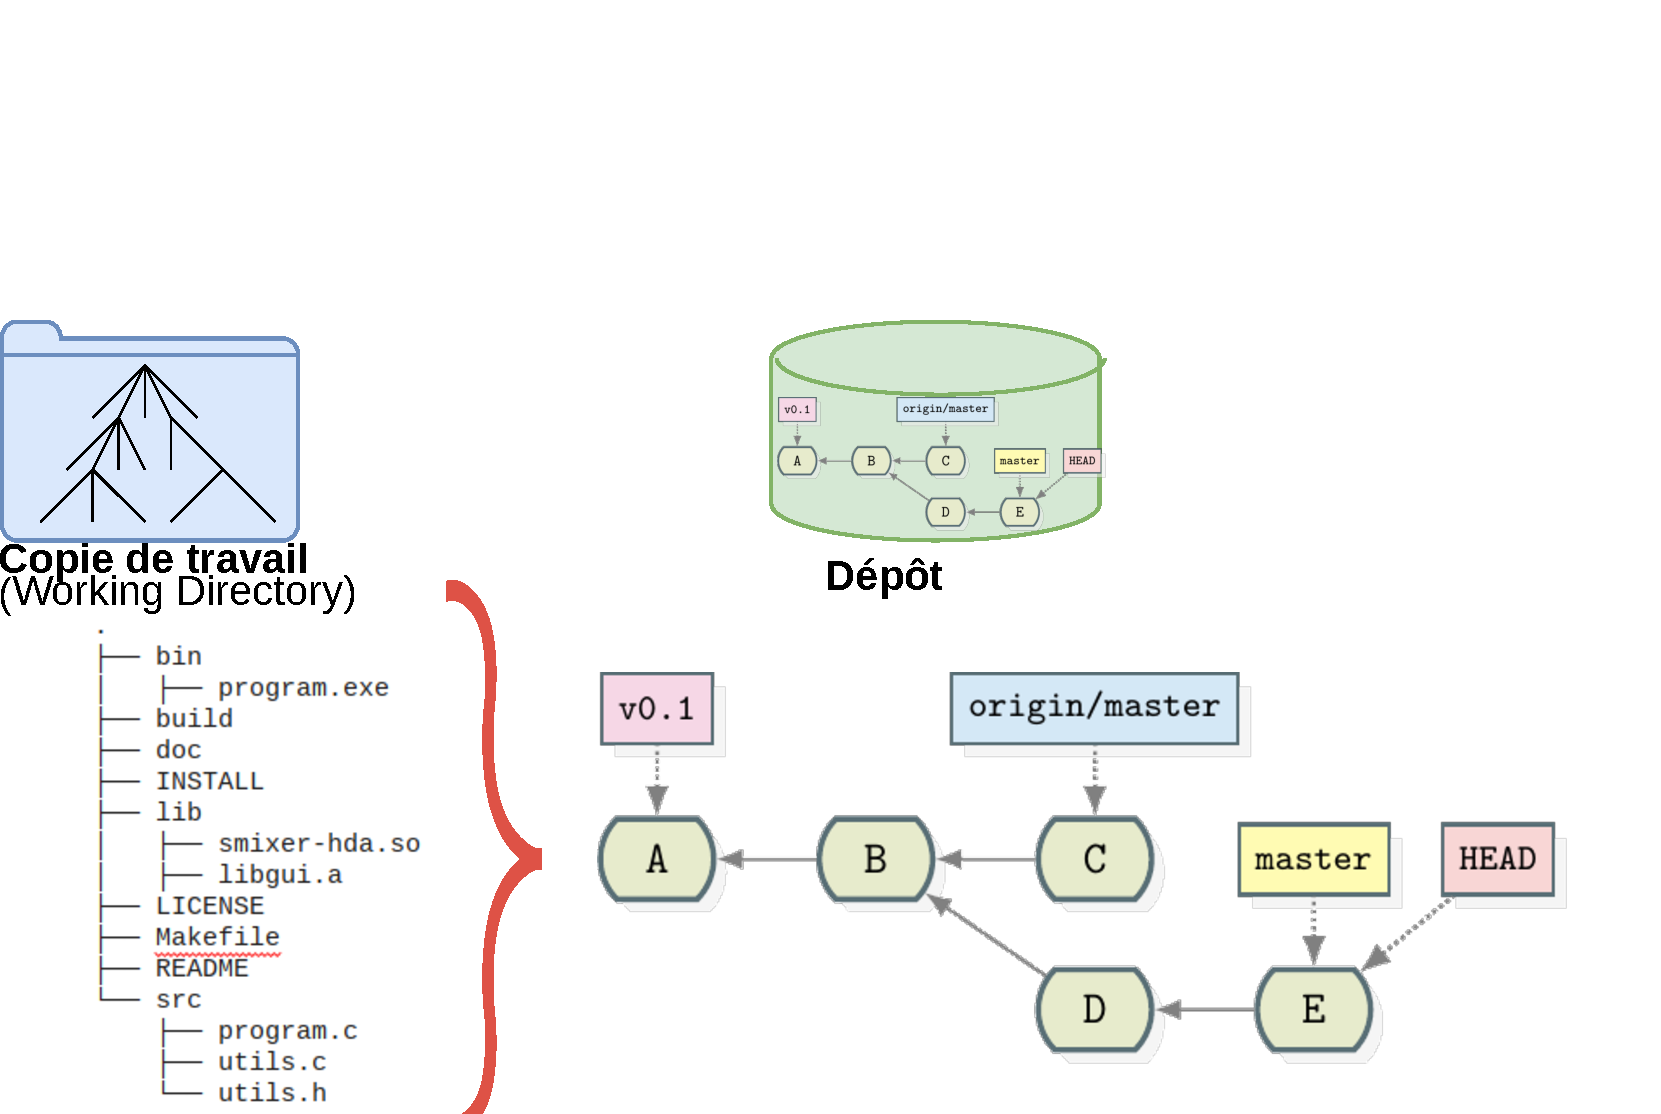
\includegraphics[scale=0.44]{images/workflow2.pdf}}}
		\only<3>{{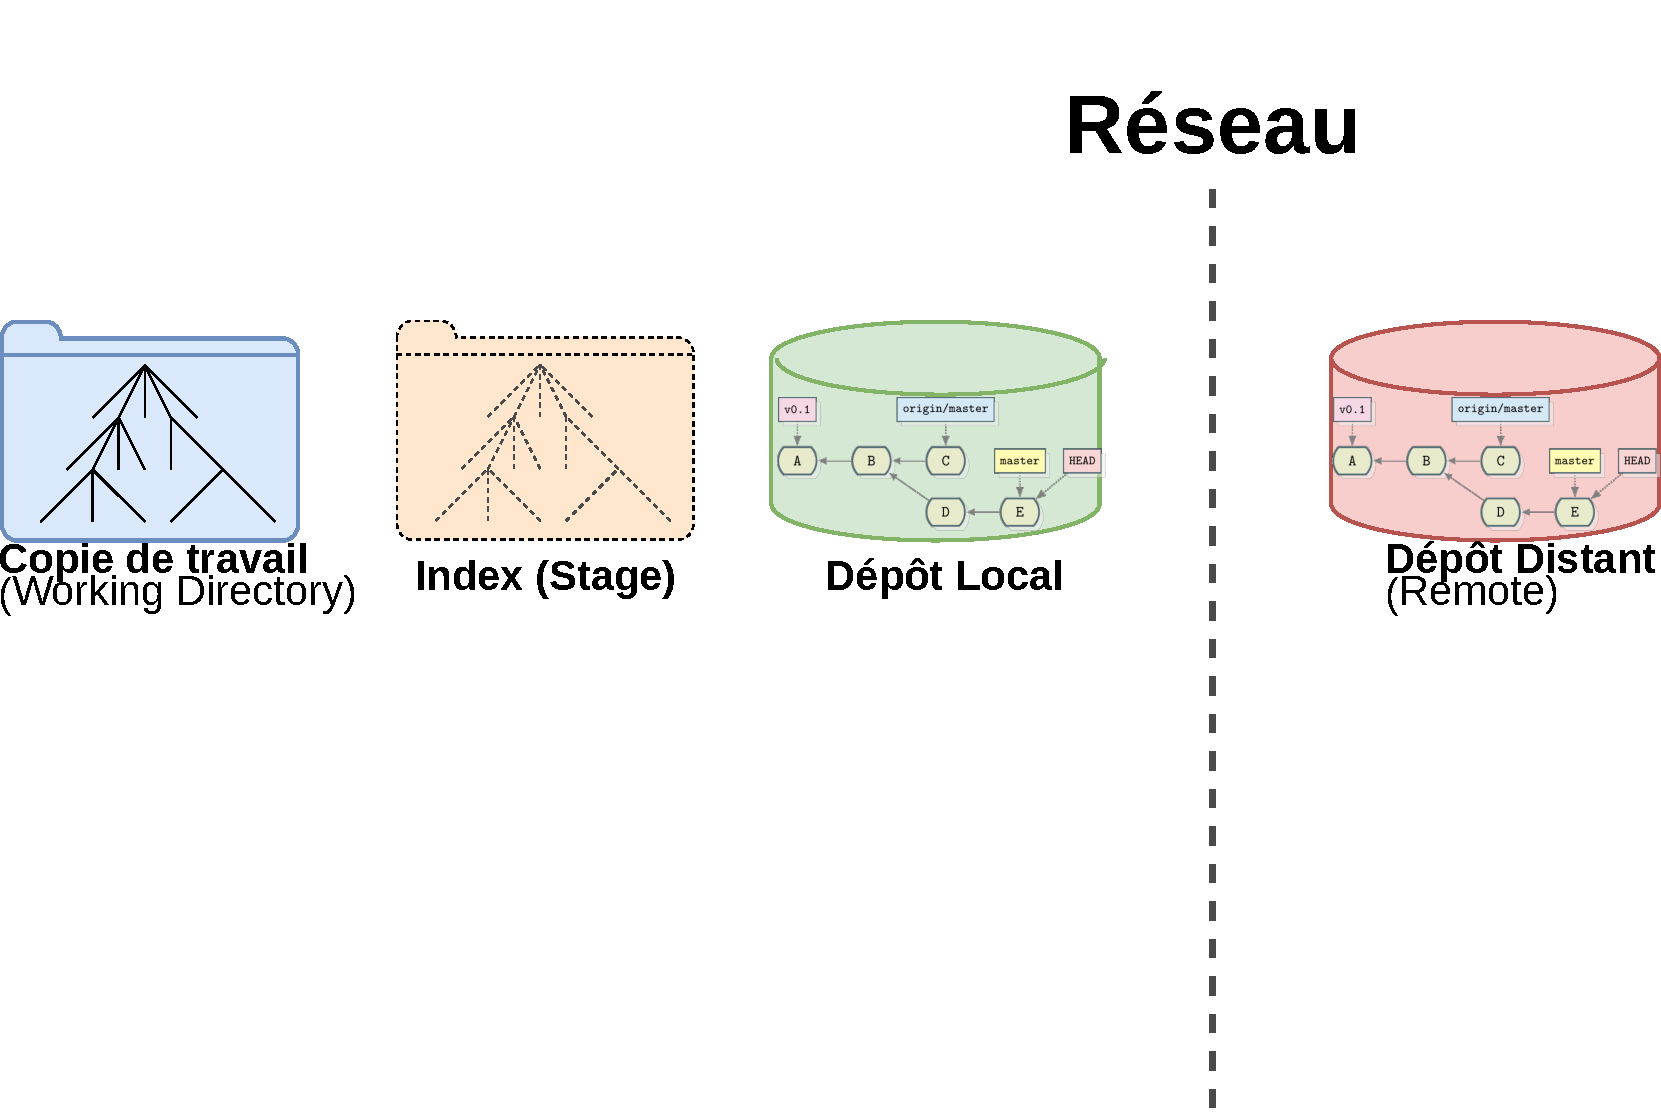
\includegraphics[scale=0.44]{images/workflow3.pdf}}}
		\only<4>{{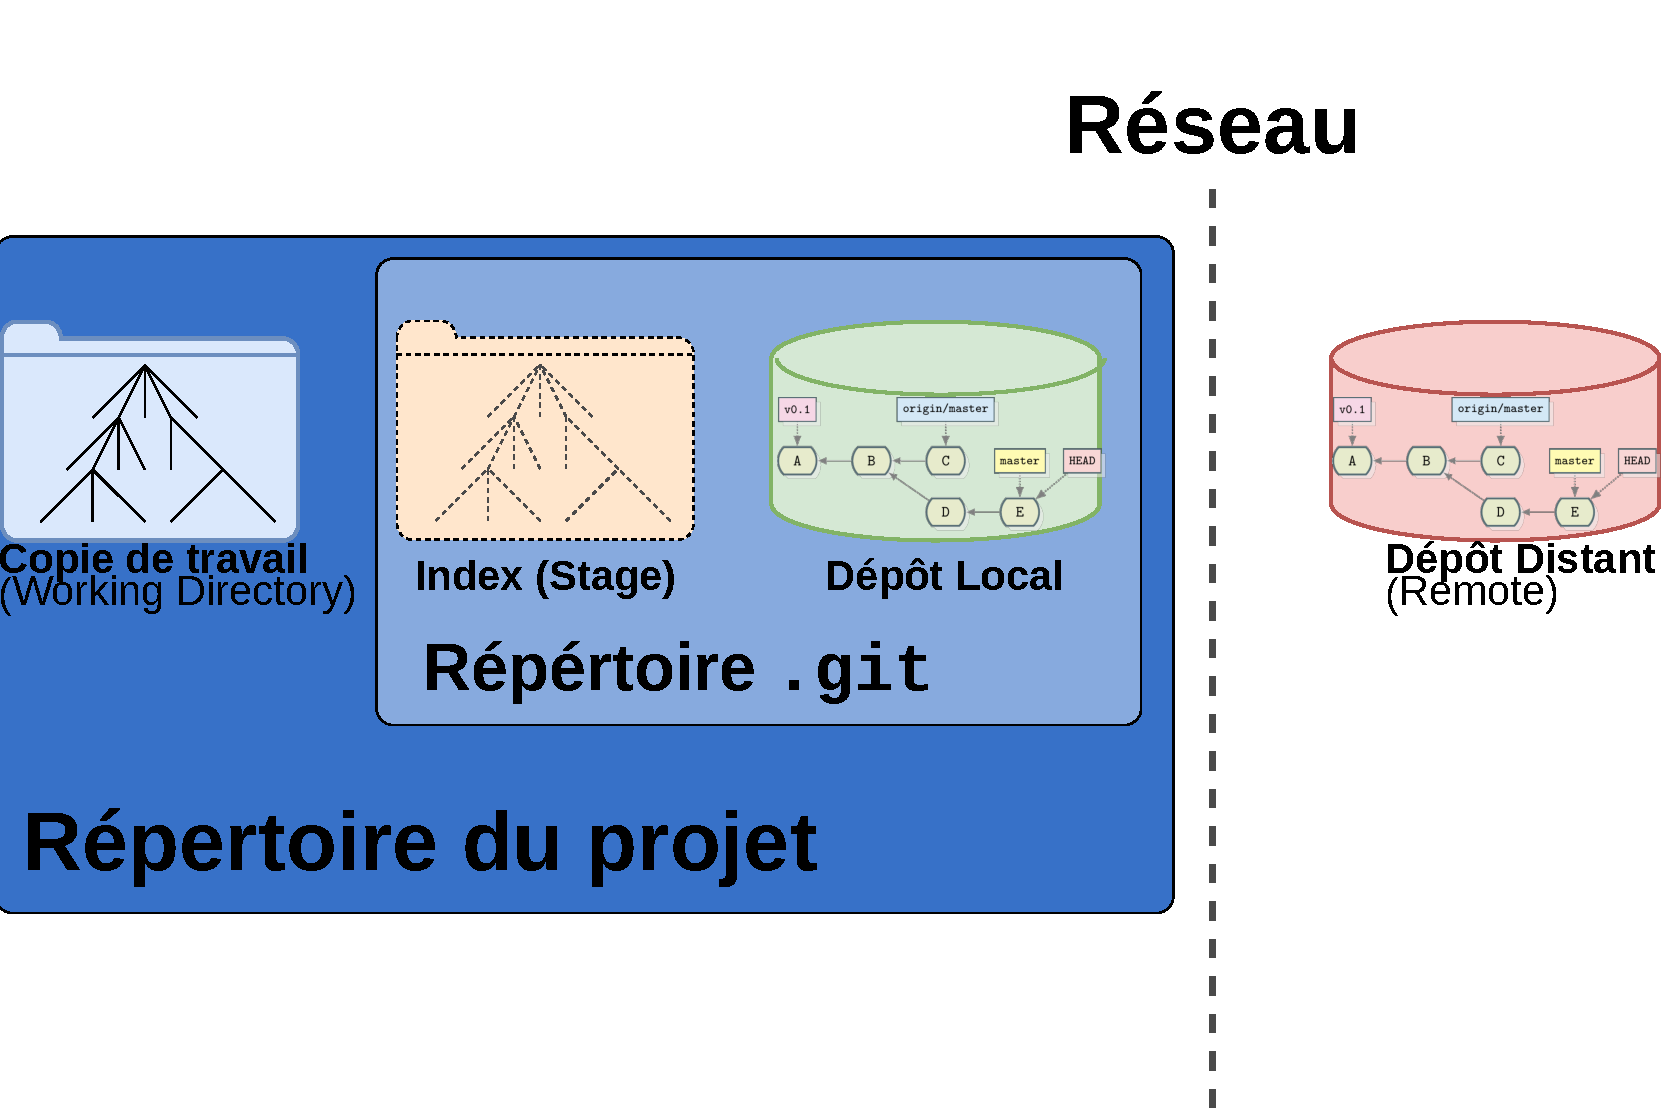
\includegraphics[scale=0.44]{images/workflow4.pdf}}}
		\only<5>{{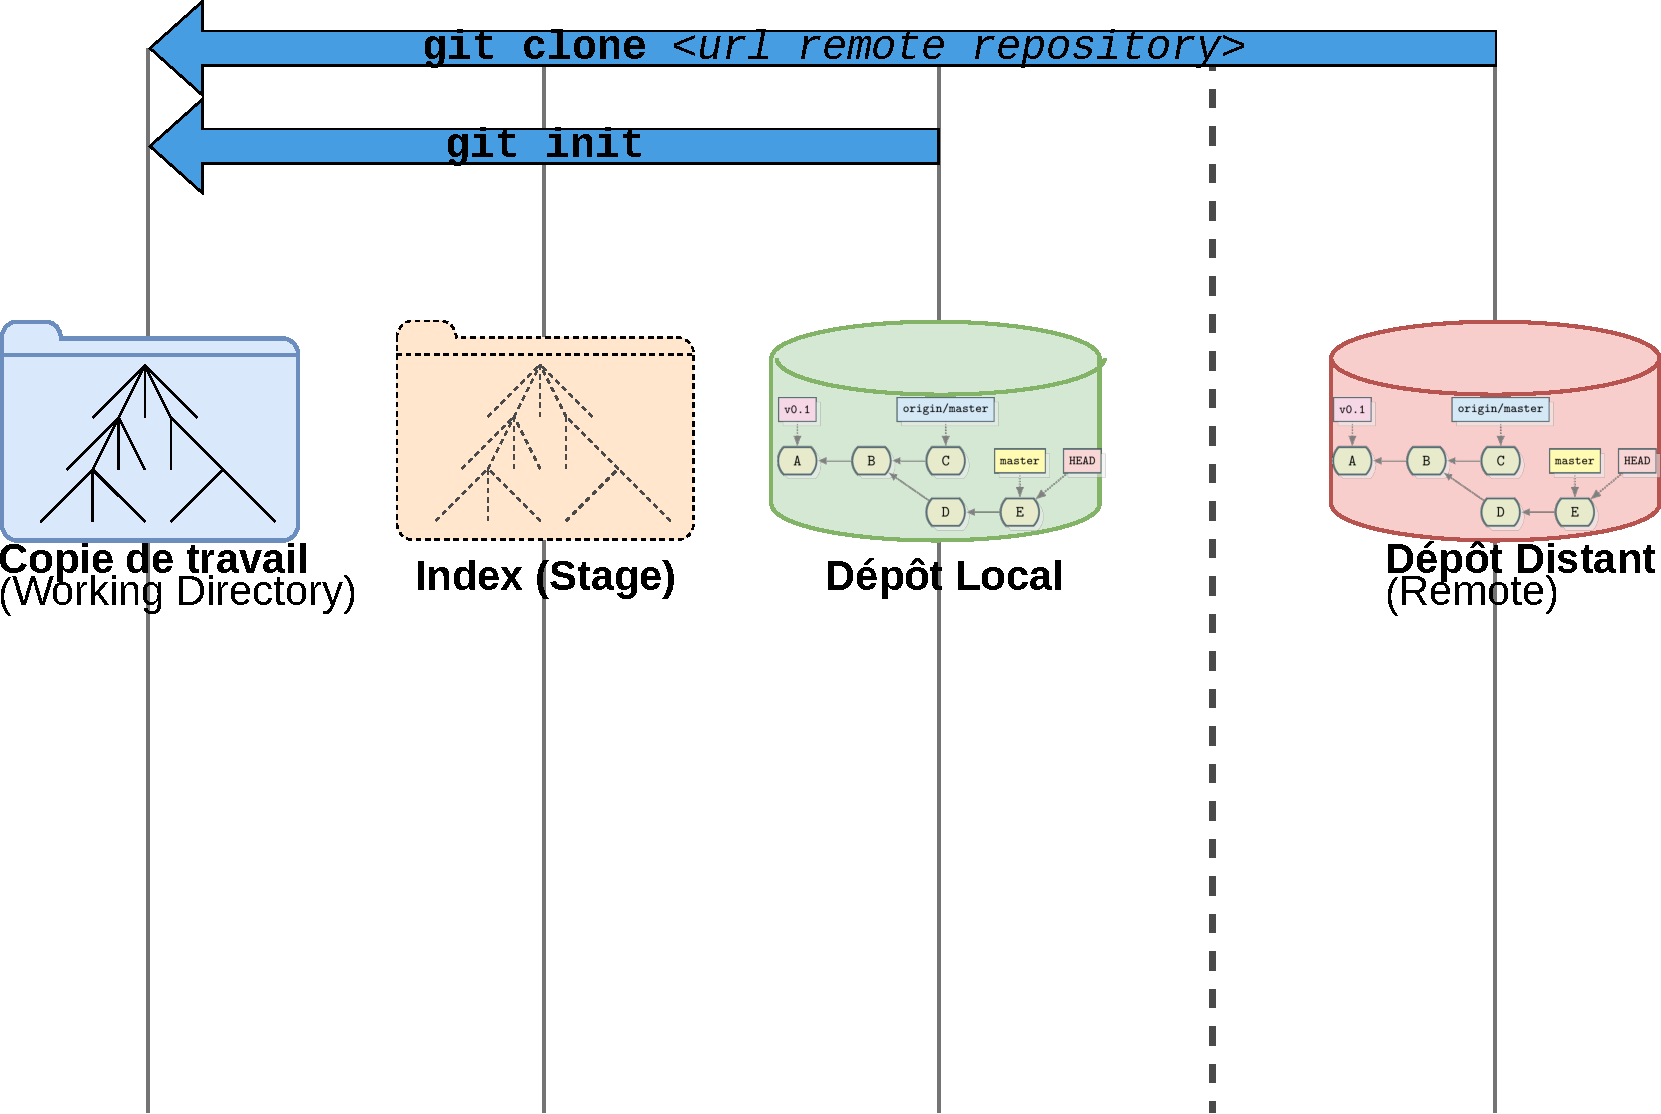
\includegraphics[scale=0.44]{images/workflow5.pdf}}}
		\only<6>{{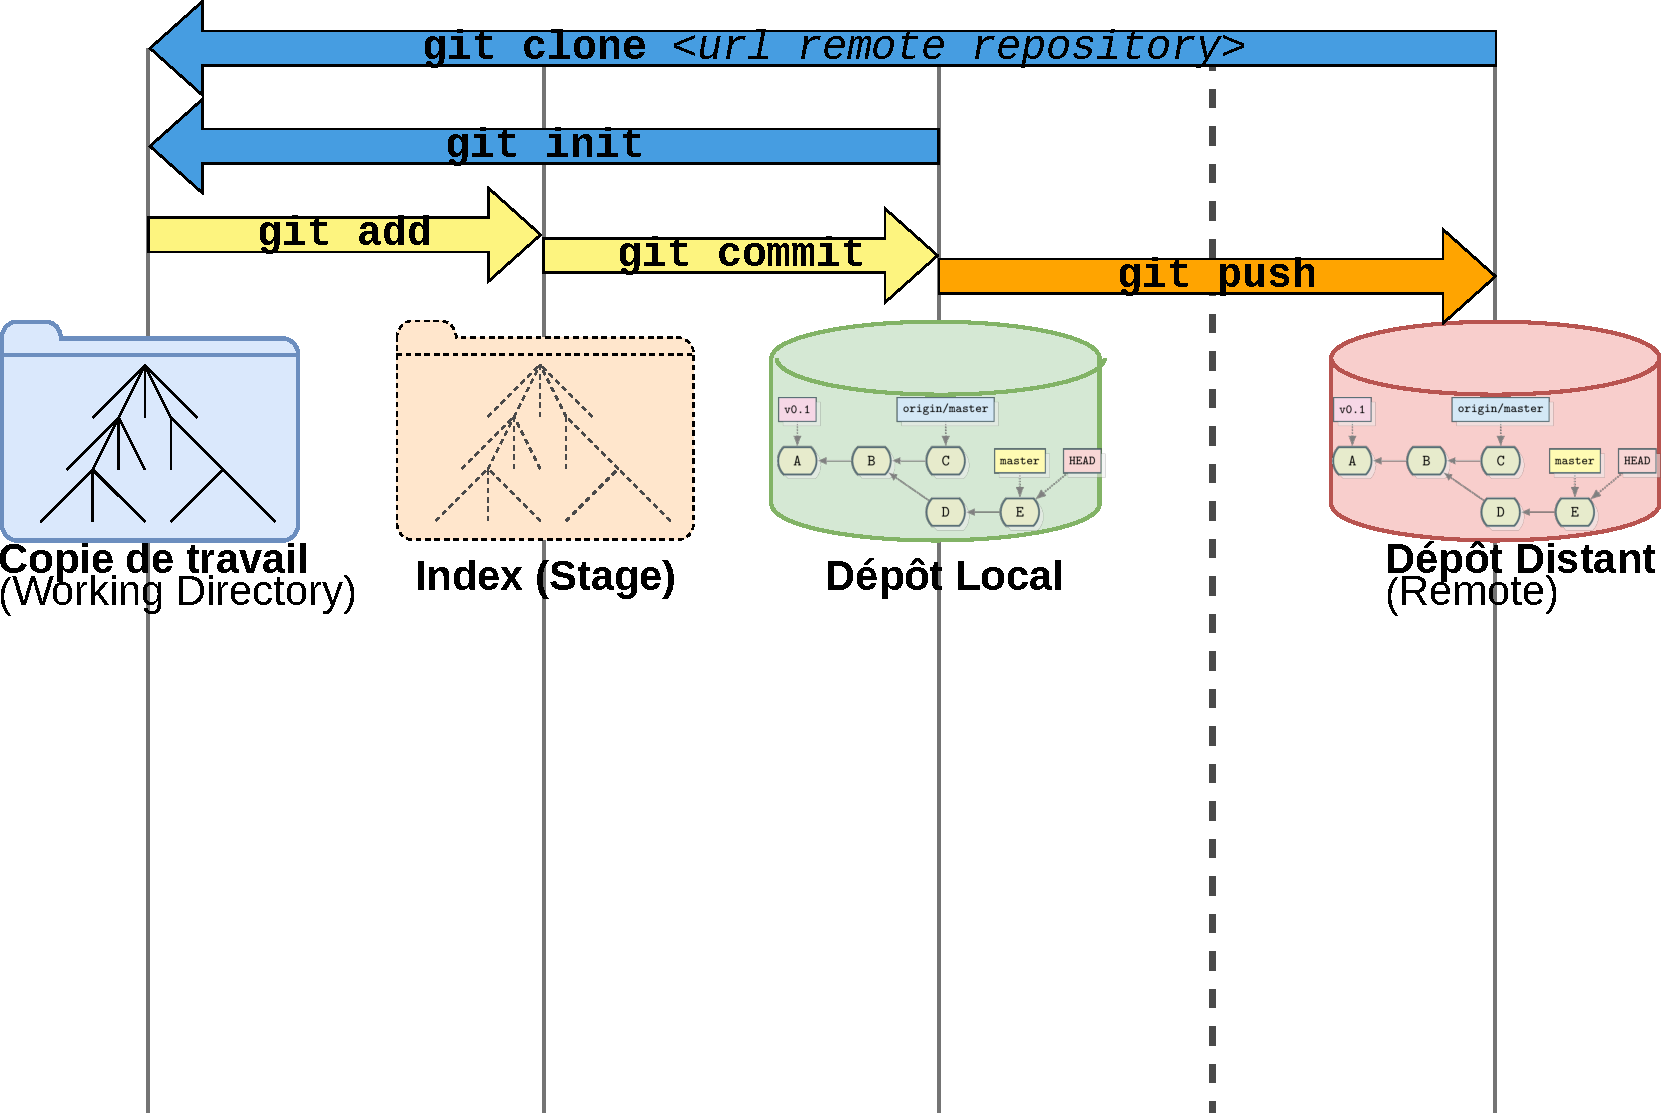
\includegraphics[scale=0.44]{images/workflow6.pdf}}}
		\only<7>{{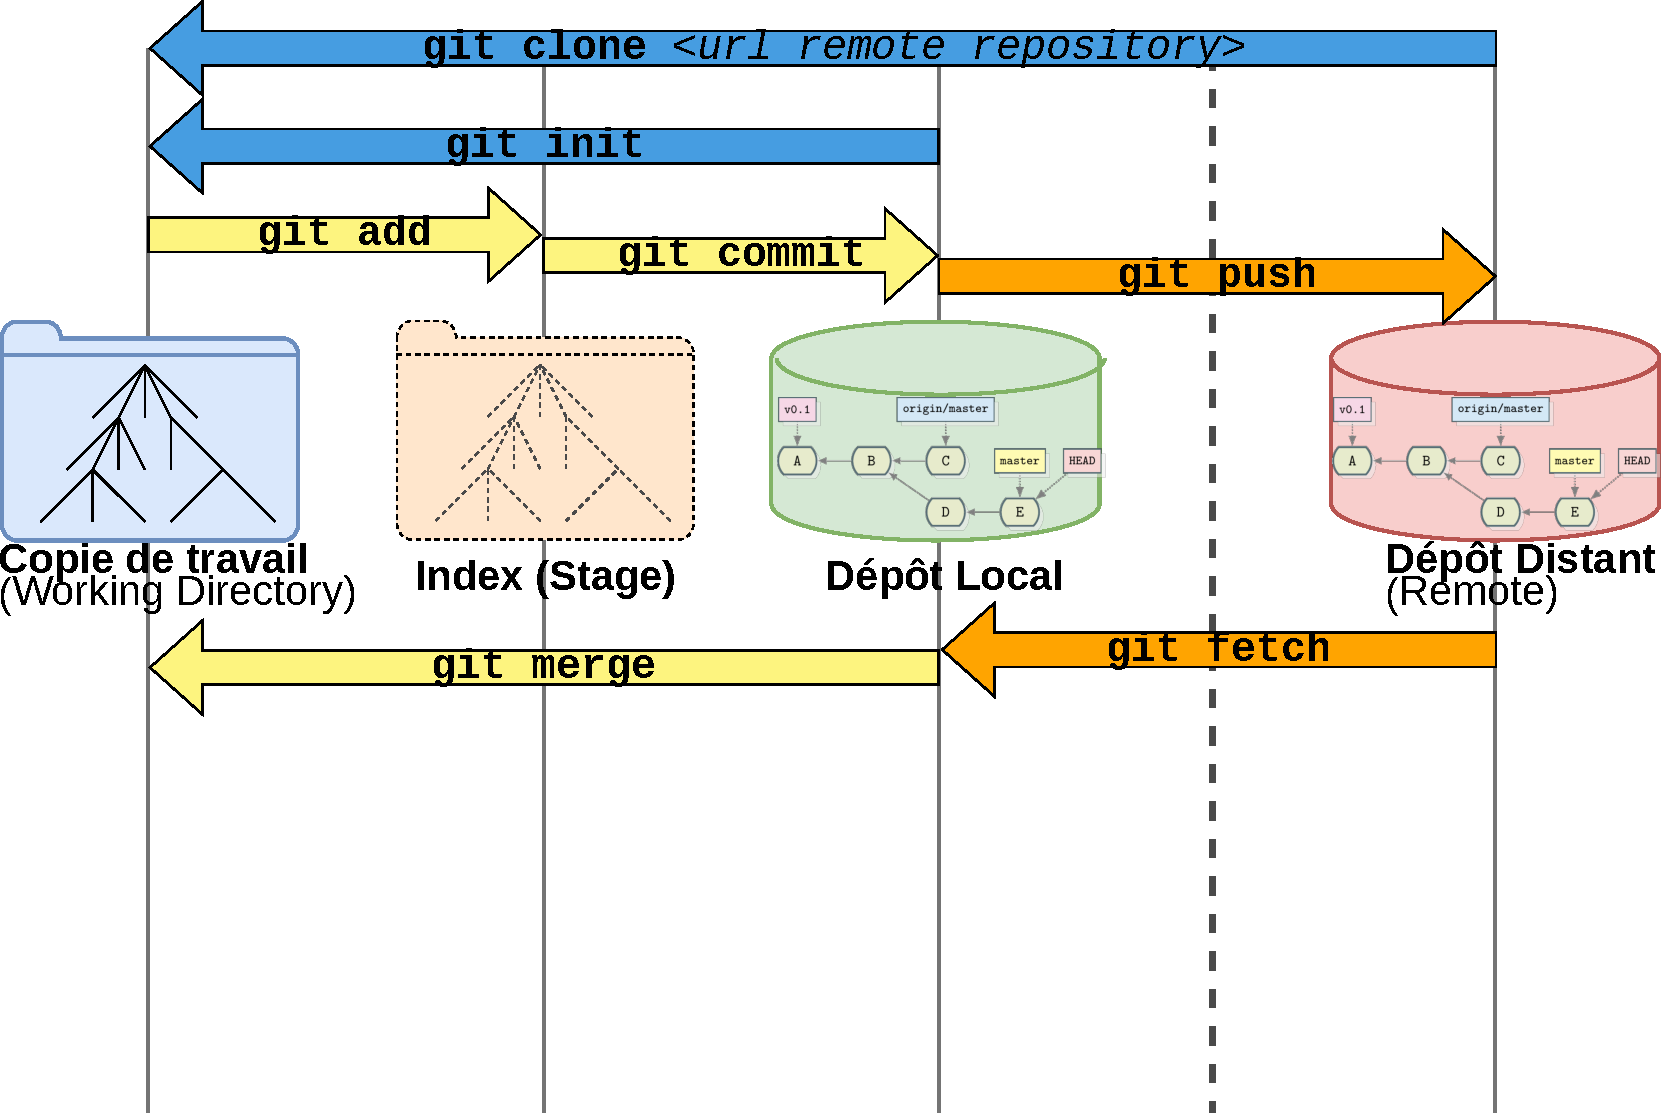
\includegraphics[scale=0.44]{images/workflow7.pdf}}}
		\only<8>{{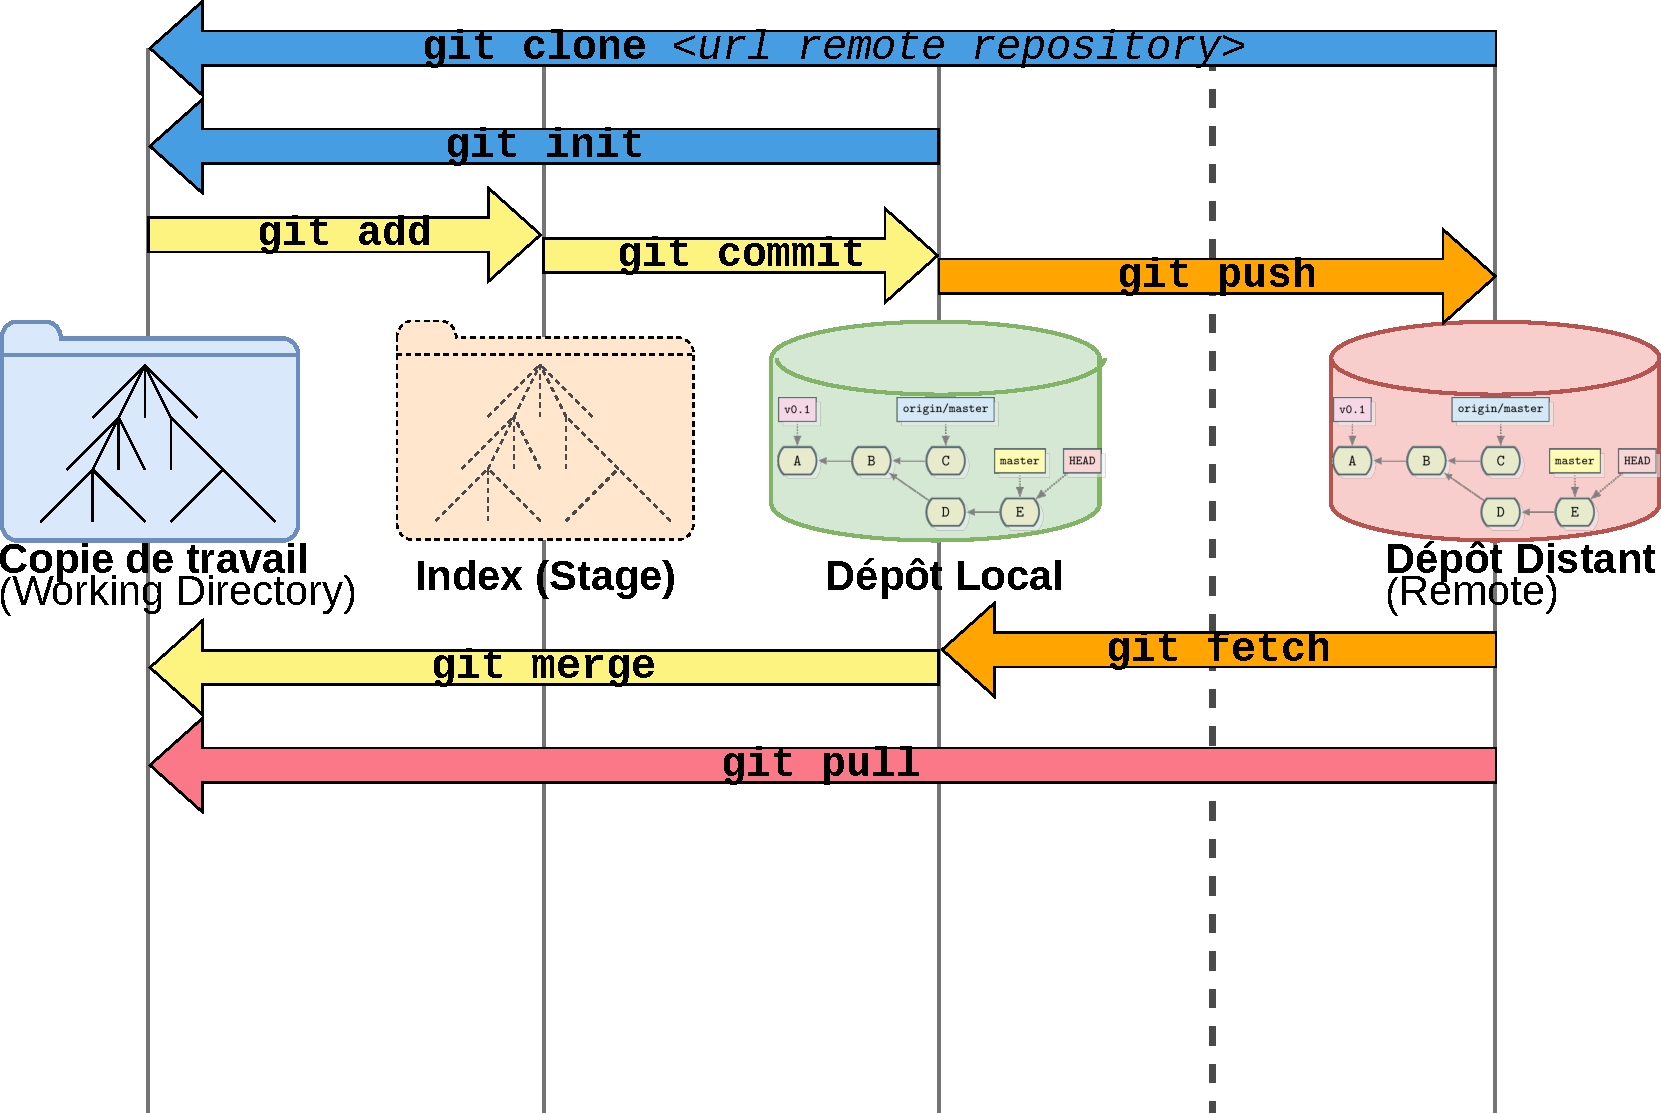
\includegraphics[scale=0.44]{images/workflow8.pdf}}}
%		\only<9>{{\includegraphics[scale=0.44]{images/workflow9.pdf}}}
%		\only<10>{{\includegraphics[scale=0.44]{images/workflow10.pdf}}}
		\only<9>{{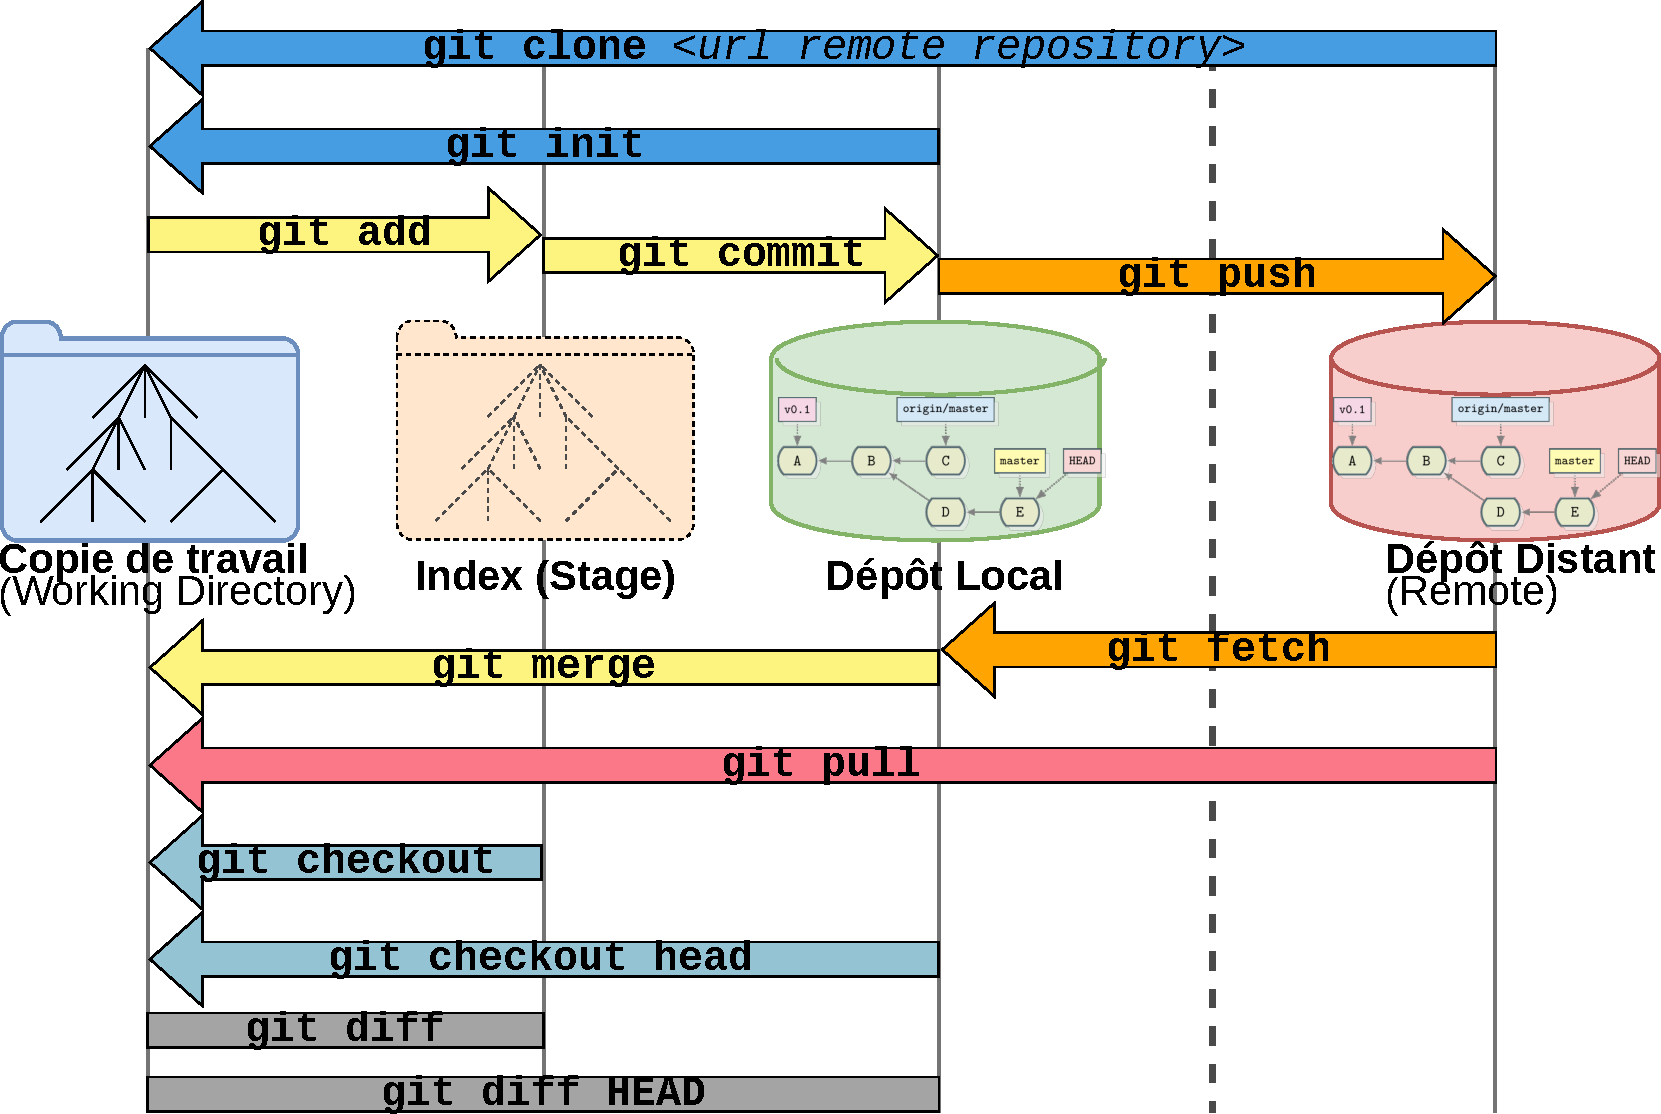
\includegraphics[scale=0.44]{images/workflow_all.pdf}}}
	\end{center}
\end{adjustwidth}
\end{frame}



%%%%%%%%%% Begin Premier Commit
\begin{frame}[fragile]
\frametitle{The Directed Acyclic \textit{Commit}-Graph in Git}
%	\vspace{-0.5cm}
 	\begin{figure}
	%\only<2->{
	\onslide<2>{
		\begin{subfigure}[h]{\textwidth}
		%\centering
		\begin{tikzpicture}
		% Commit DAG
		\gitDAG[grow right sep = 2em]{
			27ff4
		};
		% Tag reference
	%	\gittag [v0p1] {v0.1} {above=of A} {A}
		% Remote branch
		% Branch
		\gitbranch
		{master}     % node name and text 
		{above=of 27ff4} % node placement
		{27ff4}          % target
		% HEAD reference
		\gitHEAD
		%	 			{above=of master} % node placement
		{right=of master} % node placement
		{27ff4}          % target
		\end{tikzpicture}
		\end{subfigure}
	}	
	\subcaption{\only<1>{Dépôt vide}\only<2->{Premier \textit{commit}}}
	\end{figure}

%	\vspace{-0.5cm}
	\begin{block}{Dans un terminal \ldots}
	\vspace{-0.2cm}		
	\begin{minted}[mathescape=true,escapeinside=||,tabsize=4
	,fontsize=\footnotesize,
	]{c}
	mkdir mon_depot ; cd mon_depot
	git init .
	echo "pomme" |>{}>| fruits.txt
	git add fruits.txt
	git commit -m "Pomme ajouté à la liste de fruits"
	  |$\Rightarrow$| ID = 27ff4
	\end{minted}
	\end{block}
	Faire \texttt{git status} et \texttt{git log} \underline{après chaque commande}!!!
\end{frame}
%%%%%%%%%% End Premier Commit

\begin{frame}
\frametitle{C'est quoi un commit ?}
	\vspace{-1em}
	\begin{block}{}
	\begin{adjustwidth}{-0.5cm}{-0.5cm}{}
		\begin{center}	
			{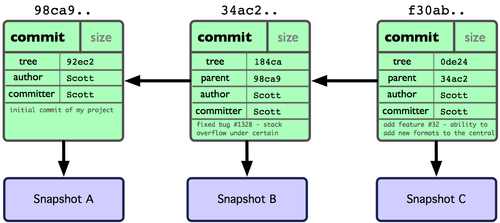
\includegraphics[scale=0.6]{images/git_commit.png}}
		\end{center}
	\end{adjustwidth}
	\end{block}

	\vspace{-2em}
	\begin{block}{}
	%    \begin{adjustwidth}{-0.9cm}{}
	\begin{itemize}
		\item Le \texttt{Commit-ID} est une \textit{empreinte} calculé en utilisant la fonction de hachage \texttt{SHA-1} sur
		\begin{itemize}
			\item \textbf{Tout} le contenu du commit + Date + Nom et email du commiteur + Message de log + ID du commit parent + \ldots
		\end{itemize}
	\end{itemize}
	%	\end{adjustwidth}
%	\begin{itemize}
%	\item 
	Propriété : \textbf{Unicité} quasi-universelle de l'\texttt{ID}
%	\begin{itemize}
%		\item Unicité universelle statistique de l'ID
%	\end{itemize}
%\end{itemize}
%	\end{adjustwidth}
\end{block}
\end{frame}


%%%%%%%%%%% ANIMATION Commit 2
\begin{frame}[fragile]
\frametitle{The DAG in Git : Commit 2}
\only<1-2>{
	\begin{figure}
		\begin{subfigure}[h]{\textwidth}
			%\centering
			\begin{tikzpicture}
			% Commit DAG
			\gitDAG[grow right sep = 2em]{
				27ff4
			};
			% Tag reference
			%	\gittag [v0p1] {v0.1} {above=of A} {A}
			% Remote branch
			% Branch
			\gitbranch
			{master}     % node name and text 
			{above=of 27ff4} % node placement
			{27ff4}          % target
			% HEAD reference
			\gitHEAD
			%	 			{above=of master} % node placement
			{right=of master} % node placement
			{27ff4}          % target
			\end{tikzpicture}
			\subcaption{État avant deuxième \texttt{commit}}
		\end{subfigure}
	\end{figure}
}

\only<3>{
	\begin{figure}
		\begin{subfigure}[h]{\textwidth}
			%\centering
			\begin{tikzpicture}
			% Commit DAG
			\gitDAG[grow right sep = 2em]{
				27ff4 -- 31490
			};
			\gitbranch
			{master}     % node name and text 
			{above=of 31490} % node placement
			{31490}          % target
			% HEAD reference
			\gitHEAD
			%	 			{above=of master} % node placement
			{right=of master} % node placement
			{31490}          % target
			\end{tikzpicture}
			\subcaption{Deuxième \textit{commit}}
		\end{subfigure}
	\end{figure}
}

%\vspace{-0.5cm}
%\vspace{0.4cm} \begin{center} \noindent\makebox[\linewidth]{\line(2,0){500}} \end{center} \vspace{-0.4cm} 
\begin{block}{Dans un terminal \ldots}<2->
%	\vspace{-0.2cm}		
	\begin{minted}[mathescape=true,escapeinside=||,tabsize=4
	,fontsize=\footnotesize,
	]{c}
	echo banane |>{}>| fruits.txt
	git add fruits.txt
	git commit -m "Ajouté banane à fruits.txt"
	  |$\Rightarrow$| ID = 31490
	\end{minted}
\end{block}

\only<2>{\begin{tikzpicture}[remember picture,overlay]\node[xshift=1cm,yshift=3.4cm] at (current page.south west) {$\hookrightarrow$};\end{tikzpicture}}
\only<3>{\begin{tikzpicture}[remember picture,overlay]\node[xshift=1cm,yshift=1.8cm] at (current page.south west) {$\hookrightarrow$};\end{tikzpicture}}

\end{frame}
%%%%%%%%%%% End ANIMATION Commit 2


%%%%%%%%%%% ANIMATION Commit 3
\begin{frame}[fragile]
\frametitle{The DAG in Git : Commit 3}

	\begin{figure}
		\begin{subfigure}[h]{\textwidth}
			%\centering
			\begin{tikzpicture}
			% Commit DAG
			\gitDAG[grow right sep = 2em]{
				27ff4 -- 31490 -- ab5d1
			};
			% Tag reference
			%	\gittag [v0p1] {v0.1} {above=of A} {A}
			% Remote branch
			% Branch
			\gitbranch
			{master}     % node name and text 
			{above=of ab5d1} % node placement
			{ab5d1}          % target
			% HEAD reference
			\gitHEAD
			%	 			{above=of master} % node placement
			{right=of master} % node placement
			{ab5d1}          % target
			\end{tikzpicture}
			\subcaption{Troisième \textit{commit}}
		\end{subfigure}
	\end{figure}

%\vspace{-0.5cm}
\begin{block}{}%Sur le terminal \ldots}
%	\vspace{-0.2cm}
	\vspace{0.4cm} \begin{center} \noindent\makebox[\linewidth]{\line(2,0){500}} \end{center} \vspace{-0.4cm} 		
	\begin{minted}[mathescape=true,escapeinside=||,tabsize=4,fontsize=\footnotesize,linenos,
	]{c}
	echo orange |>{}>| fruits.txt
	git add fruits.txt
	git commit -m "Ajouté orange à fruits.txt"
	  |$\Rightarrow$| ID = ab5d1
	\end{minted}
\end{block}
\end{frame}
%%%%%%%%%%% End ANIMATION Commit 3


%%%%%%%%%%% ANIMATION Branch 1
\begin{frame}[fragile]
\frametitle{The DAG in Git: Branches 1}
\only<1-2>{
	\begin{figure}
	\begin{subfigure}[h]{\textwidth}
		%\centering
		\begin{tikzpicture}
		% Commit DAG
		\gitDAG[grow right sep = 2em]{
			27ff4 -- 31490 -- ab5d1
		};
		% Tag reference
		%	\gittag [v0p1] {v0.1} {above=of A} {A}
		% Remote branch
		% Branch
		\gitbranch
		{master}     % node name and text 
		{above=of ab5d1} % node placement
		{ab5d1}          % target
		% HEAD reference
		\gitHEAD
		%	 			{above=of master} % node placement
		{right=of master} % node placement
		{ab5d1}          % target
		\end{tikzpicture}
		\subcaption{Avant branche}
	\end{subfigure}
	\end{figure}
}

\only<3-4>{
	\begin{figure}
	\begin{subfigure}[h]{\textwidth}
		%\centering
		\begin{tikzpicture}
		% Commit DAG
		\gitDAG[grow right sep = 2em]{
			27ff4 -- 31490 -- ab5d1
		};
		% Tag reference
		%	\gittag [v0p1] {v0.1} {above=of A} {A}
		% Remote branch
		% Branch
		\gitbranch
		{master}     % node name and text 
		{above=of ab5d1} % node placement
		{ab5d1}          % target
		% HEAD reference
		\gitHEAD
		%	 			{above=of master} % node placement
		{right=of master} % node placement
		{ab5d1}          % target
		\gitbranch {legumes} {left=of master} {ab5d1}

		\end{tikzpicture}
		\subcaption{Après branche}
		\only<3>{
		$\Rightarrow$ une nouvelle \textit{étiquette} apparait, elle pointe vers le même \texttt{commit} que \texttt{HEAD}
		\vspace{-1.65em}
		}
	\end{subfigure}
\end{figure}
}

\only<5-6>{
	\begin{figure}
		\begin{subfigure}[h]{\textwidth}
			%\centering
			\begin{tikzpicture}
			% Commit DAG
			\gitDAG[grow right sep = 2em]{
				27ff4 -- 31490 -- ab5d1 -- ffd5c
			};
			% Tag reference
			%	\gittag [v0p1] {v0.1} {above=of A} {A}
			% Remote branch
			% Branch
			\gitbranch
			{master}     % node name and text 
			{above=of ab5d1} % node placement
			{ab5d1}          % target
			% HEAD reference
			\gitHEAD
 			{below=of ffd5c} % node placement
%			{right=of legumes} % node placement
			{ffd5c}          % target
			\gitbranch {legumes} {above=of ffd5c} {ffd5c}
			
			\end{tikzpicture}
			\subcaption{Après commit dans branche \texttt{legumes}}
		\end{subfigure}
	\end{figure}
}

\only<7->{
	\begin{figure}
		\begin{subfigure}[h]{\textwidth}
			%\centering
			\begin{tikzpicture}
			% Commit DAG
			\gitDAG[grow right sep = 2em]{
				27ff4 -- 31490 -- ab5d1 -- ffd5c -- 8a928
			};
			% Tag reference
			%	\gittag [v0p1] {v0.1} {above=of A} {A}
			% Remote branch
			% Branch
			\gitbranch
			{master}     % node name and text 
			{above=of ab5d1} % node placement
			{ab5d1}          % target
			% HEAD reference
			\gitHEAD
			{below=of 8a928} % node placement
			%			{right=of legumes} % node placement
			{8a928}          % target
			\gitbranch {legumes} {above=of 8a928} {8a928}
			\end{tikzpicture}
			\subcaption{Après deuxième commit dans branche \texttt{legumes}}
		\end{subfigure}
	\end{figure}
}

%\vspace{-0.5cm}
%\only<2-3>{
%\begin{block}{Sur le terminal \ldots}

\only<2>{\begin{tikzpicture}[remember picture,overlay]\node[xshift=1cm,yshift=3.5cm] at (current page.south west) {$\hookrightarrow$};\end{tikzpicture}}
\only<3-4>{\begin{tikzpicture}[remember picture,overlay]\node[xshift=1cm,yshift=2.85cm] at (current page.south west) {$\hookrightarrow$};\end{tikzpicture}}
\only<5-6>{\begin{tikzpicture}[remember picture,overlay]\node[xshift=1cm,yshift=1.4cm] at (current page.south west) {$\hookrightarrow$};\end{tikzpicture}}
\only<7->{\begin{tikzpicture}[remember picture,overlay]\node[xshift=1cm,yshift=0.2cm] at (current page.south west) {$\hookrightarrow$};\end{tikzpicture}}


	\pause[2]
	\vspace{0.4cm} \begin{center} \noindent\makebox[\linewidth]{\line(2,0){500}} \end{center} \vspace{-0.4cm}
	\begin{minted}[mathescape=true,escapeinside=||,tabsize=4,fontsize=\footnotesize,]{c}
	git branch legumes ; git checkout legumes
	\end{minted}
	
	\pause[4]
	\begin{minted}[mathescape=true,escapeinside=||,tabsize=4,fontsize=\footnotesize,]{c}
	echo aubergine |>{}>| legumes.txt ; git add legumes.txt
	git commit -m "Ajout aubergine à legumes"
	  |$\Rightarrow$| ID = ffd5c
	\end{minted}
	\pause[6]
	\begin{minted}[mathescape=true,escapeinside=||,tabsize=4,fontsize=\footnotesize,]{c}
	echo courgette |>{}>| legumes.txt ; git add legumes.txt
	git commit -m "Ajout courgette à legumes"
	  |$\Rightarrow$| ID = 8a928
	\end{minted}
\end{frame}
%%%%%%%%%%% End ANIMATION Branch 1
%echo aubergine |>{}>| legumes.txt
%echo courgette |>{}>| legumes.txt
%git add legumes.txt
%git commit -m "Ajout de legumes"
%===> ID = ffd5c	



%%%%%%%%%%% ANIMATION Branch 2
\begin{frame}[fragile]
\frametitle{The DAG in Git: Branches 2}
\only<1>{
	\begin{figure}
		\begin{subfigure}[h]{\textwidth}
			%\centering
			\begin{tikzpicture}
			% Commit DAG
			\gitDAG[grow right sep = 2em]{
				27ff4 -- 31490 -- ab5d1 -- ffd5c -- 8a928
			};
			% Tag reference
			%	\gittag [v0p1] {v0.1} {above=of A} {A}
			% Remote branch
			% Branch
			\gitbranch
			{master}     % node name and text 
			{above=of ab5d1} % node placement
			{ab5d1}          % target
			% HEAD reference
			\gitHEAD
			{below=of 8a928} % node placement
			%			{right=of legumes} % node placement
			{8a928}          % target
			\gitbranch {legumes} {above=of 8a928} {8a928}
			
			\end{tikzpicture}
			\subcaption{Travaillons sur \texttt{master}}
		\end{subfigure}
	\end{figure}
}

\only<2-3>{
	\begin{figure}
		\begin{subfigure}[h]{\textwidth}
			%\centering
			\begin{tikzpicture}
			% Commit DAG
			\gitDAG[grow right sep = 2em]{
				27ff4 -- 31490 -- ab5d1 -- ffd5c -- 8a928
			};
			% Tag reference
			%	\gittag [v0p1] {v0.1} {above=of A} {A}
			% Remote branch
			% Branch
			\gitbranch
			{master}     % node name and text 
			{above=of ab5d1} % node placement
			{ab5d1}          % target
			% HEAD reference
			\gitHEAD
			{below=of ab5d1} % node placement
			%			{right=of legumes} % node placement
			{ab5d1}          % target
			\gitbranch {legumes} {above=of 8a928} {8a928}
			
			\end{tikzpicture}
			\subcaption{Travaillons sur \texttt{master}}
			\only<2>{$\Rightarrow$ \texttt{legumes.txt} n'existe plus dans la Copie de Travail (\textit{Working Directory})}
			\vspace{0.33em}
		\end{subfigure}
	\end{figure}
}

\only<4>{
	\begin{figure}
		\begin{subfigure}[h]{\textwidth}
			%\centering
			\begin{tikzpicture}
			% Commit DAG
			\gitDAG[grow right sep = 2em]{
				27ff4 -- 31490 -- ab5d1 -- {ffd5c -- 8a928, 21721}
			};
			% Tag reference
			%	\gittag [v0p1] {v0.1} {above=of A} {A}
			% Remote branch
			% Branch
			\gitbranch
			{master}     % node name and text 
			{below=of 21721} % node placement
			{21721}          % target
			% HEAD reference
			\gitHEAD
			{right=of master} % node placement
			%			{right=of legumes} % node placement
			{21721}          % target
			\gitbranch {legumes} {above=of 8a928} {8a928}
			
			\end{tikzpicture}
			\subcaption{Après nouveau \textit{commit} sur \texttt{master}}
			\vspace{-3em}
		\end{subfigure}
	\end{figure}
}

%\vspace{-0.5cm}
%\only<2-3>{
%\begin{block}{Sur le terminal \ldots}
%\pause[2]
%\vspace{-0.2cm}
\vspace{0.4cm} \begin{center} \noindent\makebox[\linewidth]{\line(2,0){500}} \end{center} \vspace{-0.4cm}
\begin{minted}[mathescape=true,escapeinside=||,tabsize=4,fontsize=\footnotesize,]{c}
	git checkout master
\end{minted}

\only<1>{\begin{tikzpicture}[remember picture,overlay]\node[xshift=1cm,yshift=2.6cm] at (current page.south west) {$\hookrightarrow$};\end{tikzpicture}}
\only<2>{\begin{tikzpicture}[remember picture,overlay]\node[xshift=1cm,yshift=2cm] at (current page.south west) {$\hookrightarrow$};\end{tikzpicture}}
\pause[3]
\begin{minted}[mathescape=true,escapeinside=||,tabsize=4,fontsize=\footnotesize,]{c}
	echo poire |>{}>| fruits.txt ; git add fruits.txt
	git commit -m "Ajouté poire à fruits.txt"
		|$\Rightarrow$| ID = 21721
\end{minted}
\only<3>{\begin{tikzpicture}[remember picture,overlay]\node[xshift=1cm,yshift=1.9cm] at (current page.south west) {$\hookrightarrow$};\end{tikzpicture}}
\only<4->{\begin{tikzpicture}[remember picture,overlay]\node[xshift=1cm,yshift=0.6cm] at (current page.south west) {$\hookrightarrow$};\end{tikzpicture}}
\end{frame}
%%%%%%%%%%% End ANIMATION Branch 2


%%%%%%%%%%% ANIMATION Merge 1
\begin{frame}[fragile]
\frametitle{The DAG in Git: Merge 1}
\only<1-2>{
	\begin{figure}
		\begin{subfigure}[h]{\textwidth}
			%\centering
			\begin{tikzpicture}
			% Commit DAG
			\gitDAG[grow right sep = 1.5em]{
				27ff4 -- 31490 -- ab5d1 -- {ffd5c -- 8a928, 21721}
			};
			% Tag reference
			%	\gittag [v0p1] {v0.1} {above=of A} {A}
			% Remote branch
			% Branch
			\gitbranch
			{master}     % node name and text 
			{below=of 21721} % node placement
			{21721}          % target
			% HEAD reference
			\gitHEAD
			{right=of legumes} % node placement
			%			{right=of legumes} % node placement
			{8a928}          % target
			\gitbranch {legumes} {above=of 8a928} {8a928}
			
			\end{tikzpicture}
			\subcaption{Allons sur \texttt{légumes}, regardons les différences}
			%\only<2>{$\Longrightarrow$ \texttt{legumes.txt} n'existe plus dans \textit{Working Directory})}
		\end{subfigure}
	\end{figure}
}

\only<3>{
	\begin{figure}
		\begin{subfigure}[h]{\textwidth}
			%\centering
			\begin{tikzpicture}
			% Commit DAG
			\gitDAG[grow right sep = 1.5em]{
				27ff4 -- 31490 -- ab5d1 -- {ffd5c -- 8a928, 21721} -- 760cf
			};
			% Tag reference
			%	\gittag [v0p1] {v0.1} {above=of A} {A}
			% Remote branch
			% Branch
			\gitbranch
			{master}     % node name and text 
			{below=of 21721} % node placement
			{21721}          % target
			% HEAD reference
			\gitHEAD
			{above=of 760cf} % node placement
			%			{right=of legumes} % node placement
			{760cf}          % target
			\gitbranch {legumes} {left=of gitHEAD} {760cf}
			
			\end{tikzpicture}
			\subcaption{Merger \texttt{master} dans \texttt{légumes} : produit un \underline{nouveau commit}}
			%\only<2>{$\Longrightarrow$ \texttt{legumes.txt} n'existe plus dans \textit{Working Directory})}
		\end{subfigure}
	\end{figure}
}


%\vspace{-0.5cm}
%\only<2-3>{
%\begin{block}{Sur le terminal \ldots}
%\pause[2]
%\vspace{-0.2cm}
\vspace{0.4cm} \begin{center} \noindent\makebox[\linewidth]{\line(2,0){500}} \end{center} \vspace{-0.4cm}
\begin{minted}[mathescape=true,escapeinside=||,tabsize=4,fontsize=\footnotesize,]{c}
	git checkout legumes
\end{minted}

\only<1>{\begin{tikzpicture}[remember picture,overlay]\node[xshift=1cm,yshift=1.7cm] at (current page.south west) {$\hookrightarrow$};\end{tikzpicture}}

\pause[2]
\begin{minted}[mathescape=true,escapeinside=||,tabsize=4,fontsize=\footnotesize,]{c}
	git diff master
\end{minted}

\only<2>{\begin{tikzpicture}[remember picture,overlay]\node[xshift=1cm,yshift=1.1cm] at (current page.south west) {$\hookrightarrow$};\end{tikzpicture}}

\pause[3]
\begin{minted}[mathescape=true,escapeinside=||,tabsize=4,fontsize=\footnotesize,]{c}
	git merge master
\end{minted}
\only<3>{\begin{tikzpicture}[remember picture,overlay]\node[xshift=1cm,yshift=0.5cm] at (current page.south west) {$\hookrightarrow$};\end{tikzpicture}}
\end{frame}
%%%%%%%%%%% End ANIMATION Merge 1

\begin{frame}[fragile]
\frametitle{Merge 1 : Vue dans la console}
%\begin{block}{Représentation par pointeurs}%Parcours postfixé ou \texttt{GRD}}
\begin{adjustwidth}{-1cm}{-0.8cm}{}
	\begin{center}
		{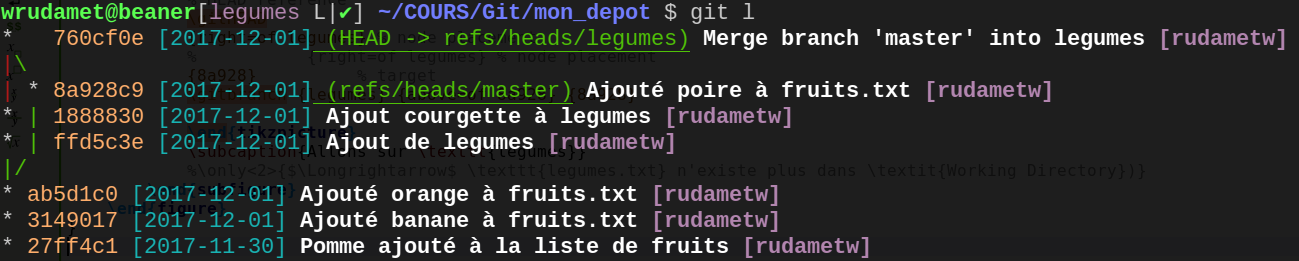
\includegraphics[scale=0.3]{images/git_log_merge.png}}
		\begin{minted}[mathescape=true,escapeinside=||,tabsize=4,fontsize=\footnotesize,]{c}
			git log |-{}-|all |-{}-|graph |-{}-|oneline |-{}-|date=short
		\end{minted}
	\end{center}
\end{adjustwidth}
%\end{block}
\end{frame}



%%%%%%%%%%% ANIMATION Merge 2
\begin{frame}[fragile]
\frametitle{The DAG in Git: Merge 2}
\only<1>{
	\begin{figure}
		\begin{subfigure}[h]{\textwidth}
			%\centering
			\begin{tikzpicture}
			% Commit DAG
			\gitDAG[grow right sep = 1.5em]{
				27ff4 -- 31490 -- ab5d1 -- {ffd5c -- 8a928, 21721} -- 760cf
			};
			% Tag reference
			%	\gittag [v0p1] {v0.1} {above=of A} {A}
			% Remote branch
			% Branch
			\gitbranch
			{master}     % node name and text 
			{below=of 21721} % node placement
			{21721}          % target
			% HEAD reference
			\gitHEAD
			{right=of master} % node placement
			%			{right=of legumes} % node placement
			{21721}          % target
			\gitbranch {legumes} {above=of 760cf} {760cf}
			
			\end{tikzpicture}
			\subcaption{Allons sur \texttt{master}}
			%\only<2>{$\Longrightarrow$ \texttt{legumes.txt} n'existe plus dans \textit{Working Directory})}
		\end{subfigure}
	\end{figure}
}

\only<2>{
	\begin{figure}
		\begin{subfigure}[h]{\textwidth}
			%\centering
			\begin{tikzpicture}
			% Commit DAG
			\gitDAG[grow right sep = 1.5em]{
				27ff4 -- 31490 -- ab5d1 -- {ffd5c -- 8a928, 21721} -- 760cf
			};
			% Tag reference
			%	\gittag [v0p1] {v0.1} {above=of A} {A}
			% Remote branch
			% Branch
			\gitbranch
			{master}     % node name and text 
			{below=of 760cf} % node placement
			{760cf}          % target
			% HEAD reference
			\gitHEAD
			{left=of legumes} % node placement
			%			{right=of legumes} % node placement
			{760cf}          % target
			\gitbranch {legumes} {above=of 760cf} {760cf}
			
			\end{tikzpicture}
			\subcaption{Merger \texttt{légumes} dans \texttt{master} : \underline{pas de nouveau commit}}
			%\only<2>{$\Longrightarrow$ \texttt{legumes.txt} n'existe plus dans \textit{Working Directory})}
		\end{subfigure}
	\end{figure}
}

\only<3>{
	\begin{figure}
		\begin{subfigure}[h]{\textwidth}
			%\centering
			\begin{tikzpicture}
			% Commit DAG
			\gitDAG[grow right sep = 1.5em]{
				27ff4 -- 31490 -- ab5d1 -- {ffd5c -- 8a928, 21721} -- 760cf
			};
			% Tag reference
			%	\gittag [v0p1] {v0.1} {above=of A} {A}
			% Remote branch
			% Branch
			\gitbranch
			{master}     % node name and text 
			{below=of 760cf} % node placement
			{760cf}          % target
			% HEAD reference
			\gitHEAD
			{above=of 760cf} % node placement
			%			{right=of legumes} % node placement
			{760cf}          % target
%			\gitbranch {legumes} {above=of 760cf} {760cf}
			
			\end{tikzpicture}
			\subcaption{Effacer la branche \texttt{légumes}}
			%\only<2>{$\Longrightarrow$ \texttt{legumes.txt} n'existe plus dans \textit{Working Directory})}
		\end{subfigure}
	\end{figure}
}
\vspace{0.4cm} \begin{center} \noindent\makebox[\linewidth]{\line(2,0){500}} \end{center} \vspace{-0.4cm}

\only<1>{\vspace{0.5em}}
\begin{minted}[mathescape=true,escapeinside=||,tabsize=4,fontsize=\footnotesize,]{c}
	git checkout master
\end{minted}

\only<1>{\begin{tikzpicture}[remember picture,overlay]\node[xshift=1cm,yshift=1.8cm] at (current page.south west) {$\hookrightarrow$};\end{tikzpicture}}

\pause[2]
\begin{minted}[mathescape=true,escapeinside=||,tabsize=4,fontsize=\footnotesize,]{c}
	git diff legumes
	git merge legumes
\end{minted}
\only<2>{\begin{tikzpicture}[remember picture,overlay]\node[xshift=1cm,yshift=1.3cm] at (current page.south west) {$\hookrightarrow$};\end{tikzpicture}}
\pause
\begin{minted}[mathescape=true,escapeinside=||,tabsize=4,fontsize=\footnotesize,]{c}
	git branch -d legumes
\end{minted}
\only<3->{\begin{tikzpicture}[remember picture,overlay]\node[xshift=1cm,yshift=0.7cm] at (current page.south west) {$\hookrightarrow$};\end{tikzpicture}}
\end{frame}
%%%%%%%%%%% End ANIMATION Merge 2



%\begin{frame}{TODO: Origin}
%
%All previous parts show how the graph is constructed locally.
%
%TODO: EXPLAIN HOW TO PUSH/PULL BETWEEN DIFFERENT REPOSITORIES.
%MERGING, KEEPING UP TO DATE, ORIGIN/MASTER TAG.
%
%This should describe how the "distributed" part of Git Works.
%
%%\begin{minted}[mathescape=true,escapeinside=||,tabsize=4
%%	%,fontsize=\footnotesize,
%%	]{c}
%%	echo "pommes" |>{}>| fruits.txt
%%\end{minted}
%\end{frame}


\begin{frame}{Partager : dépôts distants}
\begin{adjustwidth}{-0.75cm}{0cm}{}
\vspace{-1em}
	\begin{center}
		\only<1>{{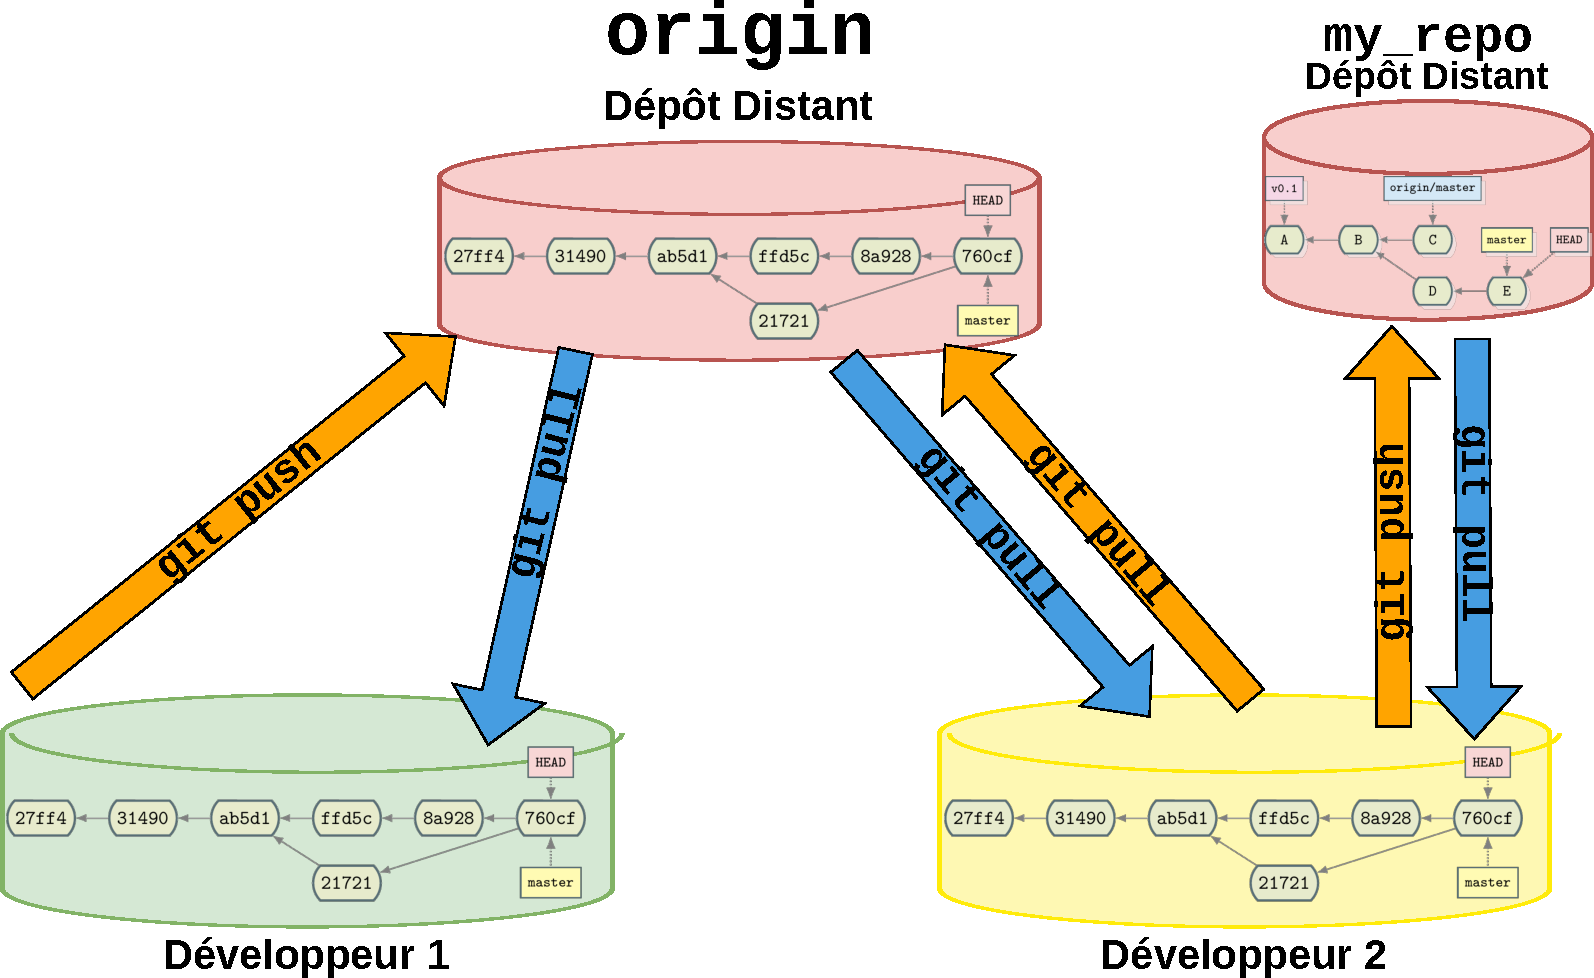
\includegraphics[scale=0.44]{images/remote_origin.pdf}}}
	\end{center}
\end{adjustwidth}
\end{frame}



%%%%%%%%%%%%%%%%%%%%%%%%%%%%%%%%%%%%%%%%%%%%%%%%%%%%%%%%%%%%%%%%%%%%%%%%%%%%%%%%%%%%%%%%%%%%%%

\begin{frame}
\frametitle{Git distribué : Développements distribués}

\begin{figure}
%	\hfill
	\centering
	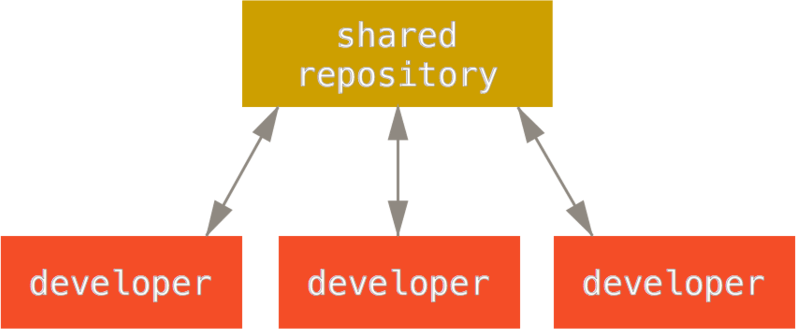
\includegraphics[scale=0.3]{images/centralized_workflow-trim.png}\\
	\small Centralized
\end{figure}

\vspace{-1em}
\color{gray}\rule{\linewidth}{2pt}
\pause
\begin{adjustwidth}{-2cm}{-1cm}{}
	\begin{columns}[T] % align columns
		\begin{column}{.5\textwidth}
			\begin{figure}
%				\hfill
				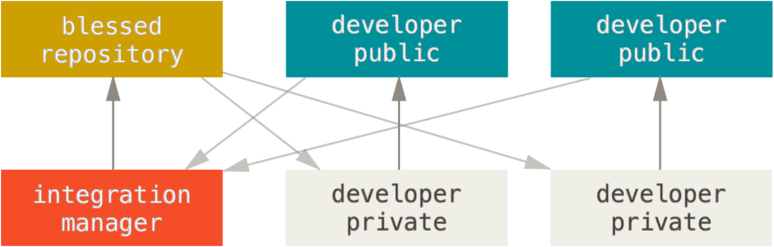
\includegraphics[scale=0.22]{images/integration-manager-trim.png}
				\small {Integration manager}
			\end{figure}
		\end{column}%
%		\hfill%
		\begin{column}{.6\textwidth}
			\vspace{-0.35em}
			\begin{figure}
				\hfill%
				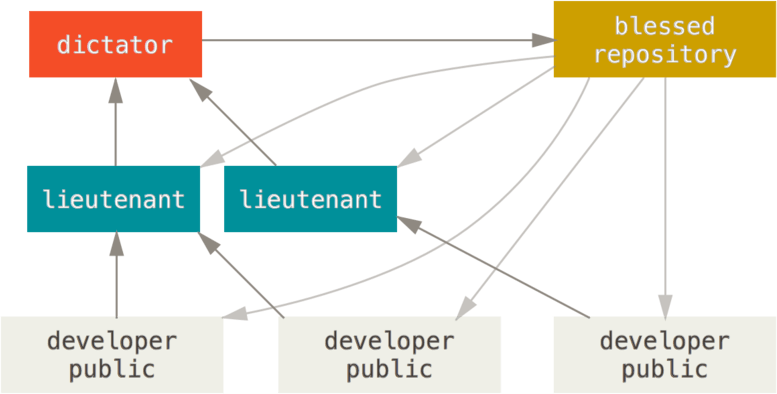
\includegraphics[scale=0.23]{images/benevolent-dictator-trim.png}
				Benevolent Dictator
			\end{figure}
		\end{column}%
	\end{columns}
\end{adjustwidth}
\end{frame}

%%%%%%%%%%%%%%%%%%%%%%%%%%%%%%%%%%%%%%%%%%%%%%%%%%%%%%%%%%%%%%%%%%%%%%%%%%%%%%%%%%%%%%%%%%%%%%
\begin{frame}[fragile]
\frametitle{Git distribué : Gestion Centralisée}
\begin{adjustwidth}{-2em}{0cm}{}
\color{darkgreen}%\rule{\linewidth}{4pt}
\noindent
Premier commit \\ \small(dépôt central doit être créé et vide)
\color{black}
\end{adjustwidth}
\begin{adjustwidth}{-1em}{0cm}{}
\begin{minted}[mathescape=true,escapeinside=**,tabsize=4,fontsize=\footnotesize,linenos,breaklines,
numbersep=5pt,
]{c}
git init .
git add .
git commit -m "first commit"

git remote add origin git@github.com:rudametw/Learning-Git-Test-Repo.git
git push -u origin master
\end{minted}
\end{adjustwidth}

\begin{adjustwidth}{-0cm}{0cm}{}
	\begin{columns}[T] % align columns
		\begin{column}{.6\textwidth}
		\end{column}%
		%\hfill%
%		\color{darkgreen}\rule{\linewidth}{4pt}
		\begin{column}{.3\textwidth}
%			\color{blue}\rule{\linewidth}{4pt}
%			Workflow \textit{(édité à la main)}
			\color{black}
			\vspace{-11em}
			\begin{adjustwidth}{-0cm}{-3cm}{}
				\begin{figure}
					\hfill
					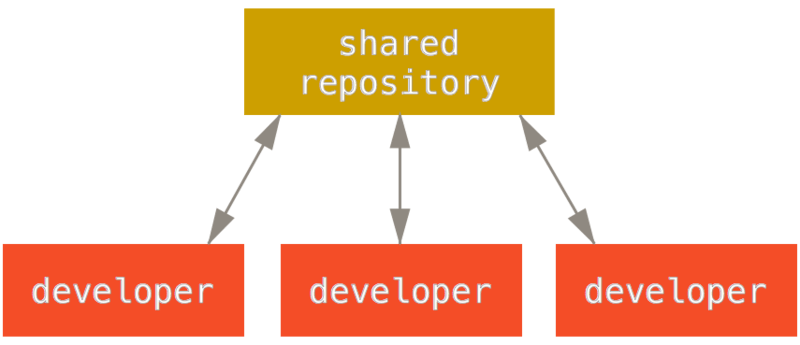
\includegraphics[scale=0.22]{images/centralized_workflow.png}
				\end{figure}
			\end{adjustwidth}
		\end{column}%
	\end{columns}
	\vspace{-1em}
	\pause
	\color{darkgray}\rule{\linewidth}{2pt}
%	\begin{columns}[T] % align columns
%	\begin{column}{.5\textwidth}
	
	\begin{adjustwidth}{-0.5cm}{-3cm}{}
		\color{darkgreen}%\rule{\linewidth}{4pt}
		Chaque développeur \texttt{clone} une seule fois
		\color{black}
		\begin{minted}[mathescape=true,escapeinside=**,tabsize=4,fontsize=\footnotesize,linenos,
		numbersep=5pt,
		]{c}
git clone https://github.com/rudametw/Learning-Git-Test-Repo.git
cd Learning-Git-Test-Repo/
git remote -v //permet de vérifier les addresses
		\end{minted}
		\end{adjustwidth}
	\end{adjustwidth}
\end{frame}

%%%%%%%%%%%%%%%%%%%%%%%%%%%%%%%%%%%%%%%%%%%%%%%%%%%%%%%%%%%%%%%%%%%%%%%%%%%%%%%%%%%%%%%%%%%%%%
%continue previous slide, broken into two
%%%%%%%%%%%%%%%%%%%%%%%%%%%%%%%%%%%%%%%%%%%%%%%%%%%%%%%%%%%%%%%%%%%%%%%%%%%%%%%%%%%%%%%%%%%%%%

\begin{frame}[fragile]
\frametitle{Git distribué : Gestion Centralisée}
\begin{adjustwidth}{-1em}{0cm}{}
\vspace{-2.3em}
\color{darkgreen}%\rule{\linewidth}{4pt}
Chacun travaille sur une branche et merge \texttt{master} dans sa branche régulièrement. Il faut tester régulièrement, et pour finir on merge sa branche vers \texttt{master} pour partager.\\
\color{black}
\vspace{-1em}
\begin{minted}[mathescape=true,escapeinside=**,tabsize=4,fontsize=\footnotesize,linenos,breaklines,
numbersep=5pt,
]{c}
git pull ; git status //update & check work
git branch fonctionalitéX
git checkout fonctionalitéX
//while (je travaille = vrai) {
	git status
	git add XXX
	git commit XXX
//}
git pull
git merge master
//gérér conflits s'il y en a

//tester que tout marche
git checkout master
git merge fonctionalitéX
git pull ; git push
\end{minted}
\end{adjustwidth}

\vspace{-12em}

\begin{adjustwidth}{-0cm}{-1cm}{}
	\begin{figure}
		\hfill
		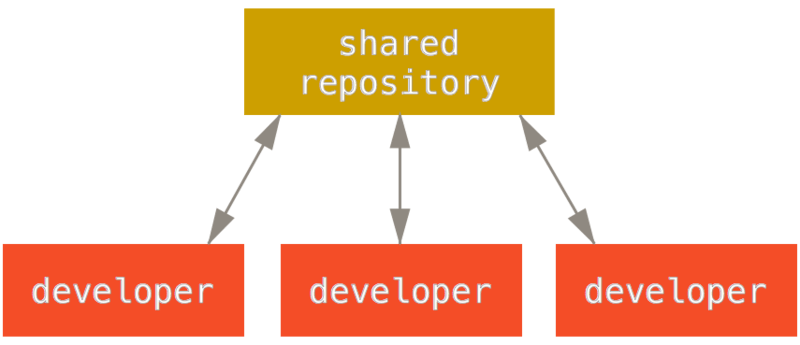
\includegraphics[scale=0.22]{images/centralized_workflow.png}
	\end{figure}
\end{adjustwidth}


\end{frame}
%%%%%%%%%%%%%%%%%%%%%%%%%%%%%%%%%%%%%%%%%%%%%%%%%%%%%%%%%%%%%%%%%%%%%%%%%%%%%%%%%%%%%%%%%%%%%%

\begin{frame}
\frametitle{Résolution de conflits}
\begin{block}{Des conflits vont se produire \ldots}
\end{block}
\begin{block}{\ldots comment faire pour les résoudre ?}
\end{block}
\end{frame}

%%%%%%%%%%%%%%%%%%%%%%%%%%%%%%%%%%%%%%%%%%%%%%%%%%%%%%%%%%%%%%%%%%%%%%%%%%%%%%%%%%%%%%%%%%%%%%

\begin{frame}[fragile]
\frametitle{Provoquer un conflit dans \texttt{fruits.txt}}
\begin{adjustwidth}{-0.3cm}{-0.3cm}{}
\vspace{-0.2em}
\begin{columns}[T] % align columns
	\begin{column}{.52\textwidth}
%		\vspace{0.5em}
		\color{darkgreen}
%		{\rule{\linewidth}{3pt}}
		Branche \texttt{ananas}
%		\vspace{+0.4em}
		\color{black}
\begin{minted}[mathescape=true,escapeinside=||,tabsize=4,fontsize=\footnotesize,breaklines]{bash}
git checkout master
git branch ananas
git checkout ananas
awk 'NR==3\{print "ananas"\}1' fruits.txt > fruits.txt
git add fruits.txt
git commit -m "+ananas"
\end{minted}
	\end{column}%
	\hfill%
	\begin{column}{.52\textwidth}
		\vspace{-0.2em}
		\color{blue}%\rule{\linewidth}{4pt}
%		+ \texttt{kaki} et - \texttt{orange}
		Branche \texttt{kaki}
		\color{black}
		\vspace{-0.3em}
\begin{minted}[tabsize=4,fontsize=\footnotesize,linenos,breaklines, numbersep=30pt,]{bash}
git checkout master
git branch kaki
git checkout kaki
awk 'NR==3\{print kaki\}1' fruits.txt | grep -v orange > fruits.txt
git add fruits.txt
git commit -m "+kaki -orange"
\end{minted}
\end{column}%
\end{columns}
\end{adjustwidth}

\color{gray}\rule{\linewidth}{3pt}
\color{black}
\vspace{-0.82em}

\begin{adjustwidth}{0.4cm}{-1cm}{}
	\vspace{-0.48em}
	\begin{columns}[T] % align columns
		\begin{column}{.45\textwidth}
\color{darkgreen}%\rule{\linewidth}{4pt}
Les merges
\color{black}
\begin{minted}[tabsize=4,fontsize=\footnotesize,linenos,breaklines,
numbersep=5pt,
]{c}
git branch merge_fruits
git checkout merge_fruits
git merge ananas
\end{minted}
\end{column}%
\hfill%
\begin{column}{.6\textwidth}

\color{darkgreen}%\rule{\linewidth}{4pt}
Sorties console
\color{black}
\vspace{-1em}
\begin{minted}[tabsize=4,fontsize=\footnotesize,breaklines,
bgcolor=mintedbackground,
]{c}
Updating 760cf0e..1711864
Fast-forward
fruits.txt | 1 +
1 file changed, 1 insertion(+)
\end{minted}
\end{column}%
\end{columns}

%\vspace{-em}
%	\hspace{0.6cm}
\begin{columns}[T] % align columns
	\hspace{0.3cm}
	\begin{column}{.3\textwidth}
		\color{darkgreen}%\rule{\linewidth}{4pt}
%		Deuxième merge
		\color{black}
		\begin{minted}[tabsize=4,fontsize=\footnotesize,linenos,breaklines,firstnumber=4,
		numbersep=5pt,
		]{text}
git merge kaki
		\end{minted}
		
	\end{column}%
%	\hfill%
	\hspace{-0.4cm}
	\begin{column}{.9\textwidth}
		
	\color{darkgreen}%\rule{\linewidth}{4pt}
%		\textit{Sortie console des merges}
	\color{black}
	\vspace{-0.2em}
	\begin{minted}[mathescape=true,escapeinside=||,tabsize=4,fontsize=\footnotesize,breaklines,
	bgcolor=mintedbackground,
	]{c}
Auto-merging fruits.txt
CONFLICT (content): Merge conflict in fruits.txt
Automatic merge failed; fix conflicts and then commit the result.
		\end{minted}
	\end{column}%
\end{columns}
\end{adjustwidth}
\end{frame}

%%%%%%%%%%%%%%%%%%%%%%%%%%%%%%%%%%%%%%%%%%%%%%%%%%%%%%%%%%%%%%%%%%%%%%%%%%%%%%%%%%%%%%%%%%%%%%

\begin{frame}
\frametitle{\texttt{diff} entre \texttt{ananas} et \texttt{kaki} avant de merger}
%\begin{block}{Représentation par pointeurs}%Parcours postfixé ou \texttt{GRD}}
\begin{adjustwidth}{-0.8cm}{-0.8cm}{}
	\begin{figure}
		\centering
		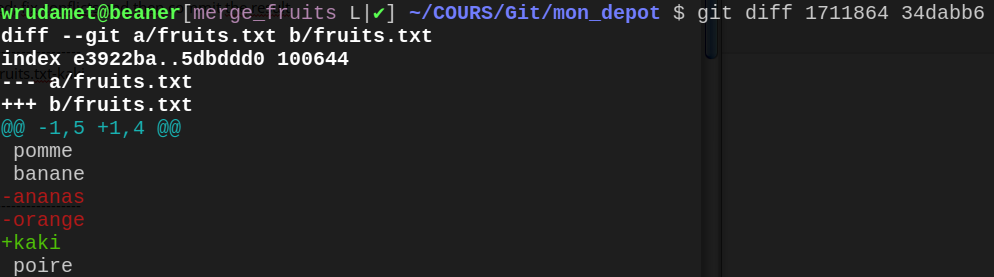
\includegraphics[scale=0.35]{images/git_diff_conflict.png}
		{Différences entre les \textit{commits} réalisés sur les branches \texttt{kaki} et \texttt{ananas} qui avaient pour objectif de produire un conflit. En {\color{red}rouge}, les lignes qui existent sur la branche \texttt{ananas} et pas \texttt{kaki}. En {\color{green}vert} les lignes qui éxistent sur la branche \texttt{kaki} et pas \texttt{ananas}.}
		\label{figure:example}
	\end{figure}
\end{adjustwidth}
%\end{block}
\end{frame}

%%%%%%%%%%%%%%%%%%%%%%%%%%%%%%%%%%%%%%%%%%%%%%%%%%%%%%%%%%%%%%%%%%%%%%%%%%%%%%%%%%%%%%%%%%%%%%

\begin{frame}[fragile]
\frametitle{Résoudre un conflit dans \texttt{fruits.txt}\\
\small immédiatement après la commande \texttt{git merge kaki}}
\begin{adjustwidth}{0cm}{-0.8cm}{}
%	\vspace{-0.6em}
	\begin{columns}[T] % align columns
		\begin{column}{.55\textwidth}
			\color{darkgreen}%\rule{\linewidth}{4pt}
			\noindent
			Conflit dans \texttt{fruits.txt} \\ {\footnotesize\texttt{git} ajoute des guides pour s'y retrouver}
			\color{black}
			\begin{minted}[mathescape=true,escapeinside=**,tabsize=4,fontsize=\footnotesize,linenos,breaklines,
			numbersep=5pt,
			]{c}
pomme
banane
*<{}<{}<{}<{}<{}<{}<* HEAD
ananas
orange
||||||| merged common ancestors
orange
=======
kaki
*>{}>{}>{}>{}>{}>{}>*
poire
		\end{minted}
%		\hspace{-2.7cm}
		\end{column}%
%		\hfill%
		\begin{column}{.5\textwidth}
			\color{darkgreen}%\rule{\linewidth}{4pt}
			Solution \textit{(édité à la main)}
			\color{black}
%			\vspace{-1em}
			\begin{minted}[tabsize=4,fontsize=\footnotesize,breaklines,linenos,
%			bgcolor=mintedbackground,
			]{c}
pomme
banane
ananas
kaki
poire
			\end{minted}
\color{gray}\rule{\linewidth}{3pt}
\color{darkgreen}%\rule{\linewidth}{4pt}
Résolution du conflit
\color{black}
%\vspace{-1.2em}			
			\begin{minted}[tabsize=4,fontsize=\footnotesize,breaklines,linenos,
%			bgcolor=mintedbackground,
			]{c}
git add fruits.txt
git status
git commit -m "Merge branch 'kaki' into merge_fruits"
git pull
git push
			\end{minted}
		\end{column}%
	\end{columns}
\end{adjustwidth}
\end{frame}
%%%%%%%%%%%%%%%%%%%%%%%%%%%%%%%%%%%%%%%%%%%%%%%%%%%%%%%%%%%%%%%%%%%%%%%%%%%%%%%%%


\begin{frame}
\frametitle{Liens, aides et outils}
\begin{itemize}
	\item Où stocker vos projets
	\begin{itemize}
		\item \url{https://archives.plil.fr/}
		\item \url{https://github.com/}
		\item \url{https://bitbucket.org/}
		\item Votre serveur perso
	\end{itemize}
	\item Tutoriels
	\begin{itemize}
		\item \url{http://www.cristal.univ-lille.fr/TPGIT/}
		\item \url{https://crypto.stanford.edu/~blynn/gitmagic/intl/fr/book.pdf}
		\item \url{https://learngitbranching.js.org/}
		\item \url{https://try.github.io/}
		\item \url{https://git-scm.com/book/fr/v2}
	\end{itemize}
	\item Vidéos
	\begin{itemize}
		\item \url{https://www.youtube.com/watch?v=OqmSzXDrJBk}
		\item \url{https://www.youtube.com/watch?v=uR6G2v_WsRA}
		\item \url{https://www.youtube.com/watch?v=3a2x1iJFJWc}
		\item \url{https://www.youtube.com/watch?v=1ffBJ4sVUb4}
		\item \url{https://www.youtube.com/watch?v=duqBHik7nRo}
	\end{itemize}
\end{itemize}
\end{frame}


% % % % % % % % % % % % % % % % % % % % % % % % % % %
% END
% % % % % % % % % % % % % % % % % % % % % % % % % % %
\end{document}
% % % % % % % % % % % % % % % % % % % % % % % % % % %
% END
% % % % % % % % % % % % % % % % % % % % % % % % % % %
